\documentclass{article}
\usepackage{graphicx} % Required for inserting images
\usepackage[utf8]{inputenc}
\usepackage{amsmath,amsfonts,amssymb,amsthm}
\usepackage{enumerate,bbm}
\usepackage{leftindex}
\usepackage{tikz,tikz-cd,graphicx,color,mathrsfs,color,hyperref,boldline}
\usepackage{caption,float}
\usepackage[a4paper,margin=1in,footskip=0.25in]{geometry}

\usepackage{listings}
\usepackage{xcolor}

\usepackage{tabularx,capt-of}

\usepackage{blindtext}
%Image-related packages
\usepackage{graphicx}
\usepackage{subcaption}
\usepackage[export]{adjustbox}
\usepackage{lipsum}

%hyperref setup
\hypersetup{
    colorlinks=true,
    linkcolor=blue,
    filecolor=magenta,      
    urlcolor=cyan,
    pdftitle={Overleaf Example},
    pdfpagemode=FullScreen,
    }

%New colors defined below
\definecolor{codegreen}{rgb}{0,0.6,0}
\definecolor{codegray}{rgb}{0.5,0.5,0.5}
\definecolor{codepurple}{rgb}{0.58,0,0.82}
\definecolor{backcolour}{rgb}{0.95,0.95,0.92}

%Code listing style named "mystyle"
\lstdefinestyle{mystyle}{
  backgroundcolor=\color{backcolour}, commentstyle=\color{codegreen},
  keywordstyle=\color{magenta},
  numberstyle=\tiny\color{codegray},
  stringstyle=\color{codepurple},
  basicstyle=\ttfamily\footnotesize,
  breakatwhitespace=false,         
  breaklines=true,                 
  captionpos=b,                    
  keepspaces=true,                 
  numbers=left,                    
  numbersep=5pt,                  
  showspaces=false,                
  showstringspaces=false,
  showtabs=false,                  
  tabsize=2
}

%"mystyle" code listing set
\lstset{style=mystyle}

\theoremstyle{definition}
\newtheorem{defn}{Definition}[section]
\newtheorem{example}[defn]{Example}
\theoremstyle{remark}
\newtheorem{rem}{Remark}
\newtheorem{remS}[section]{defn}
\theoremstyle{plain}
\newtheorem{lem}[defn]{Lemma}
\newtheorem{thm}[defn]{Theorem}
\newtheorem{prop}[defn]{Proposition}
\newtheorem{fact}[defn]{Fact}
\newtheorem{crly}[defn]{Corollary}
\newtheorem{conj}[defn]{Conjecture}

%\newtheorem*{programming*}{Programming Task}

%\newtheorem{innercustomgeneric}{\customgenericname}
%\providecommand{\customgenericname}{}
%\newcommand{\newcustomtheorem}[2]{%
%  \newenvironment{#1}[1]
%  {%
%   \renewcommand\customgenericname{#2}%
%   \renewcommand\theinnercustomgeneric{##1}%
%   \innercustomgeneric
%  }
%  {\endinnercustomgeneric}
%}

%\newcustomtheorem{question}{Question}
%\newcustomtheorem{programming}{Programming Task}

\newcommand{\NN}{\mathbb{N}}
\newcommand{\ZZ}{\mathbb{Z}}
\newcommand{\QQ}{\mathbb{Q}}
\newcommand{\RR}{\mathbb{R}}
\newcommand{\CC}{\mathbb{C}}
\newcommand{\PP}{\mathbb{P}}
\newcommand{\FF}{\mathbb{F}}
\newcommand{\Hom}{\operatorname{Hom}}
\newcommand{\im}{\operatorname{im}}
\newcommand{\id}{\operatorname{id}}
\newcommand{\Ind}{\operatorname{Ind}}
\newcommand{\Res}{\operatorname{Res}}
\newcommand{\btop}{\mathbf{Top}}
\newcommand{\bdel}{\mathbf{\Delta}}
\newcommand{\sing}{\operatorname{Sing}}
\newcommand{\bset}{\mathbf{Set}}
\newcommand{\Rmod}{\mathbf{Mod}_R}
\newcommand{\colim}{\operatorname{colim}}

\newcommand{\calD}{\mathcal{D}}

\newcommand{\sol}{\textit{Solution: }}

\title{Simplicial Homotopy Theory}
\author{Kevin}
\date{January 2025}

\begin{document}
\maketitle
\section{Introduction}
Recall basic notions from category theory
\begin{defn}
    A category $\mathscr{C}$ consists of a collection of objects, denoted $\operatorname{ob}(\mathscr C)$, and for each pair of objects $A,B$, a collection of morphisms $\Hom_{\mathscr C}(A,B)$ such that
    \begin{itemize}
        \item [(i)] There is an associative composition law of morphisms.
        \item[(ii)] For each $A\in\operatorname{ob}(\mathscr C)$, there is a distinguished element $\id_A\in\Hom_{\mathscr C}(A,A)$, which is left and right unital.
    \end{itemize}
\end{defn}
\begin{defn}
    A morphism is called an isomorphism if it has a two-sided inverse.
\end{defn}

Given a category $\mathscr{C}$, want to classify objects up to isomorphism.

For the purpose of this course, $\mathbf{Top}$ will denote the category  with objects those topological spaces that are homeomorphic to a CW complex. Morphisms are cts functions. Isomorphisms are homeomorphisms. We might attempt to classify objects in $\mathbf{Top}$ up to homeo.

A useful tool is a functor, for every integer $i$ and commutative irng $R$
\[H_i(-;R):\mathbf{Top}\to\Rmod,\ X\mapsto H_i(X;R)\]
A key ingredient in the defns of these functors is the study of cts maps from the n-simplex into $X$, as $n$ varies.

There is a factorization of functors.
\[H_i(-;R):\mathbf{Top}\to \mathbf{HoTop}\to\Rmod\]
where $\mathbf{HoTop}$ is the full subcategory of $\mathbf{Top}$ obtained by forcing homotopic cts maps to be equal (so an isomoprhism in this category is a htpy equivalence). Homotopy theory is the study of $\mathbf{HoTop}$.
\begin{rem}
    Isomorphism classes in $\mathbf{HoTop}$ can be understood via the moduli stack of formal groups and other objects in arithmetic geometry.
\end{rem}

\textbf{Question: How to think about objects in $\mathbf{HoTop}$ up to isomorphism?}

Roughly, a homotopy type consists of 
\begin{itemize}
    \item A collection of objects
    \item For every pair of objects a collection of isomorphism between them
    \item For every pair of parallel isomorphism $f,g:A\to B$ a collection of 2-isomorphisms between them.
\end{itemize}
\begin{example}
    The following shows two different homotopy types.
    \begin{figure}[H]
        \centering
        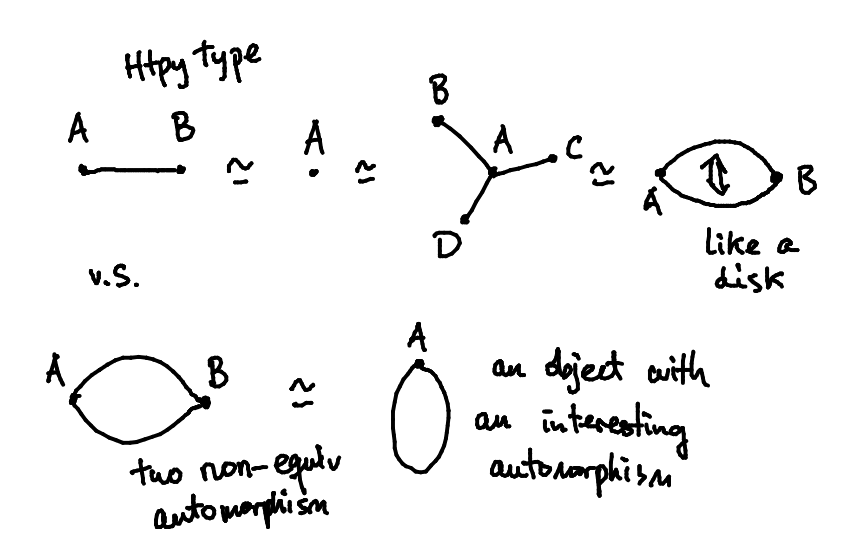
\includegraphics[width=0.5\linewidth]{Lent/pictures/htpy_type_example.PNG}
        \caption{Two different homotopy types}
        \label{fig:1}
    \end{figure}
    On the top, we have a homotopy type consisting of two objects $A, B$ and an isomorphism between them (represented by the edge). This is isomorphic to a single object $A$ as we can (formally) contract the isomorphism to identify equivalent objects. It is also equivalent to a htpy type consisting of $A,B,C,D$ where $B,C,D$ are all isomorphic to $A$ via a unique isomorphism. It is also euqivalent to the htpy type consisting of two objects $A,B$, two isomorphisms $A\to B$ and a 2-isomorphism, i.e., an equivalence of these two isomorphisms.

    On the bottom, we have another homotopy type with two objects and two non-equivalent isomorphisms. We may contract one isomoprhism and get a htpy type of consisting of a single object with an interesting automorphism.

    Sets are homotopy types with no non-trivial isomoprhisms or 2-isomorphisms.

    Groupoids, i.e., categories in which all morphisms are isomorphisms, are homotopy types with no non-trivial 2-isomorphisms and 3-isomorphisms, etc.
\end{example}
Given a topological space $X$, there is an associated homotopy type s.t.
    \begin{itemize}
        \item points of $X$ are objects. (cts maps from the $0$-simplex)
        \item paths in $X$ are isomorphisms. (cts maps from the $1$-simplex)
        \item A cts function $|\Delta^2|\to X$ is a 2-isomorphism. (Regard the map restricted to two edges of $|\Delta^2|$ as a concatenation of paths, then the map is essentially a homotopy rel the boundary of $|\Delta^1|$.)
    \end{itemize}

We want to study homotopy types. These can be presented as topological spaces (that are homeo to CW complexes) up to homotopy equivalence. SInce spaces are complicated unwieldy objects, we will seek to describe homotopy types in combinatorial terms. We will desribe homotopy types as special sorts of simplicial sets up to an appropriate notion of equivalence.

\section{Simplicial Sets}
\begin{defn}
    The simplex category $\mathbf{\Delta}$ has 
    \begin{itemize}
        \item objects $[n]$ for every integer $n\ge 0$
        \item A morphism $[n]\to[m]$ is an order preserving function from $\{1\le2\le...\le n\}\to\{1\le 2\le...\le m\}$.
    \end{itemize}
\end{defn}
There is a functor $\mathbf{\Delta}\to\mathbf{Top}$ sending $[n]\mapsto|\Delta^n|$. This is a good way to visualize $\bdel$. We introduce some special notations for certain morphisms in $\bdel$.
\begin{itemize}
    \item Face maps: $\delta^i:[n-1]\to[n]$ is the order preserving injection that omits $i$.
    \item Degeneracy maps: $\sigma^i:[n+1]\to[n]$ is the order preserving surjection that hits $i$ twice.
\end{itemize}
\begin{rem}
    Every morphism in $\bdel$ is a composite of face and degeneracy maps.
\end{rem}

\begin{defn}
    A simplicial set is a functor $\mathbf{\Delta}^{op}\to\mathbf{Set}$. A morphism of simplicial sets is a natural transformation. There is a category of simplicial sets, denoted $s\bset$.
\end{defn}
Explicitly, a simplicial set $X:\bdel^{op}\to \bset$ is a collection of sets $X_0,X_1,X_2,...$, where $X_i=X([i])$ with maps of sets $d_0,...,d_n:X_n\to X_{n-1}$ and $s_0,...,s_n:X_{n}\to X_{n+1}$ satisfying the following simplicial identities:
\begin{align*}
    &d_id_j=d_{j-1}d_i,\ \ i<j\\
    &d_is_j=s_jd_{i-1},\ \ i<j\\
    &d_is_j=s_{j}d_{i+1},\ \ i>j+1\\
    &s_is_j=s_{j+1}s_i,\ \ i<j
\end{align*}
\begin{example}
    If $X$ is a topological space, there is an associated simplicial set $\sing(X):\mathbf{\Delta}^{op}\to \mathbf{Set}$ which sends $[n]$ to the set of continuous functions $|\Delta^n|\to X$. So $\sing(X)_n=\Hom_{\btop}(|\Delta^n|,X)$.
\end{example}
\begin{rem}
    Not every simplicial set is $\sing$ of some topological space. $C_\ast^{\sing}(X;R)$ depends only on $\sing(X)$.
\end{rem}

\begin{defn}
    For every integer $n\ge 0$, there is a simplicial set denoted $\Delta^n$ defined as $(\Delta^n)_m=\Hom_\bdel([n],[m])$.
\end{defn}
Yoneda lemma implies that $\Hom_{s\bset}(\Delta^n,X)\cong X_n$ as sets for any simplicial set $X$.
\begin{rem}
    If $\mathscr{C}$ is any (small) category, the category of presheaves on $\mathscr C$ is the category of functors $\mathscr C^{op}\to\bset$. The Yoneda embedding is a functor $y:\mathscr C\to\operatorname{Psh}(\mathscr C),\ c\mapsto (c'\mapsto \Hom_{\mathscr C}(c',c))$.

    In this particular situation, $s\bset=\operatorname{Psh}(\bdel)$ and $\Delta^n=y([n])$.
\end{rem}
\begin{rem}
    Another feature of presheaf categories is that any $X\in\operatorname{Ob}(\operatorname{Psh}(\mathscr C))$ can be written as a colimit of objects in the image of the Yoneda embedding. We will appl this to $s\bset$.
\end{rem}
Let $I$ denotes the category with objects maps $\Delta^n\to X$ for any $n$ and morphisms commuting diagrams:
\begin{center}
    % https://tikzcd.yichuanshen.de/#N4Igdg9gJgpgziAXAbVABwnAlgFyxMJZABgBpiBdUkANwEMAbAVxiRAB12ARGBnOgHqEAvqXSZc+QigCM5KrUYs2ADQD6nAEZMGDGDhCjx2PASJkZC+s1aIO3XvwEBbQwphQA5vCKgAZgBOEK6IZCA4EEgATNTWyohgOgzUDHSavAAKEqbSIHp+BkYggcFIYRFIcoo2SIm6KWmZ2VJs+YVixUEhMeGRiFVxtnXJeY0MWSYtdm1uwkA
\begin{tikzcd}
\Delta^n \arrow[d] \arrow[r] & X_\bullet \\
\Delta^m \arrow[ru]          &          
\end{tikzcd}
\end{center}

Now consider the functor $I\to\bdel$, $(\Delta^n\to X_\bullet)\mapsto [n]$. Compose this with the Yoneda functor $y:\bdel\to s\bset$. We then get a functor $F:I\to s\bset$. Then $X_\bullet=\operatorname{colim}(F)$.


\begin{defn}
    Geometric realization is a functor $|\cdot |:s\bset\to\btop$.
\end{defn}
\begin{rem}
    It is the unique colimit preserving functor taking $\Delta^n$ to $|\Delta^n|$. (The previous discussion shows that if such functor exists then it's unique) We will construct this functor later :).
\end{rem}
This functor will allow us to visualize simplicial sets constructed by combinatorial means.
\begin{rem}
    If $X$ is a nice top. space, then $\sing(X)$ is a combinatorial model for the htpy type of $X$.
    Similarly, if $Y$ is a ``nice'' simplicial set, then $|Y|$ is a top. model for the htpy type of $Y$. In particular, if $X$ is a nice space then $|\sing(X)|$ is htpy equivalent to $X$.
\end{rem}
\begin{example}
    For every $n\ge0$, $\partial\Delta^n$ is a simplicial set with $(\partial \Delta^n)_m=\Hom_{s\bset}(\Delta^n,\partial\Delta^n)=\{\alpha:[m]\to[n]:\text{not surjective}\}$. There is a canonical map $\partial\Delta^n\to\Delta^n$
\end{example}
\begin{prop}
    The geometric realization $|\partial\Delta^n\to\Delta^n|$ is the inclusion of the boundary of the standard $n$-simplex.
\end{prop}
\begin{proof}
    If $n=1$, then any non-surjective order preserving function is constantly $0$ or $1$.

    If $n\ge 2$, then we have
    \[\partial \Delta^n=\operatorname{colim}\left(\coprod_{0\le i<j\le n}\Delta^{n-2}\rightrightarrows\coprod_{0\le i\le n}\Delta^{n-1}\right)\]
\end{proof}
\begin{example}
    For $n\ge1$ and $0\le i\le n$, we define $\Lambda_i^n$, the $i$th horn in $\Delta^n$ to send $[m]$ to the set of order-preserving functions $\{0\le1\le...\le m\}\to\{0\le 1\le...\le n\}$ such that $\im(\alpha)\not\supseteq\{0\le...\le i-1\}\cup\{i+1\le...\le n\}$.
    
    There is a natural map $\Lambda_i^n\to\partial\Delta^n$. The geometric realization is hte inclusion of the $i$th horn.
\end{example}

\begin{prop}
    Suppose $X$ is a topological space. For every $n\ge 1$, $0\le i\le n$ and cts map $|\Lambda_i^n\to X|$, there exists a commuting diagram in $\btop$.
    \begin{center}
        % https://tikzcd.yichuanshen.de/#N4Igdg9gJgpgziAXAbVABwnAlgFyxMJZABgBpiBdUkANwEMAbAVxiRAB8AdTgGToFsARlDoB9LAD0w7EAF9S6TLnyEUARnJVajFmwAachSAzY8BImTVb6zVog7cAIjAY46UmbK0woAc3hEoABmAE4Q-EhkIDgQSBratkhgTAwM1Ax0gi4ACkpmqiAMMEE4hsFhEYhRMUgATNQ2uojJqemZOXkqbEUlZSCh4XXUNYjxjXYtaYXtDLmmXfY9pelYYHYgInAAFj5yFLJAA
\begin{tikzcd}
\vert\Lambda_i^n\vert \arrow[r] \arrow[d] & X \\
\vert\Delta^n\vert \arrow[ru, dashed]     &  
\end{tikzcd}
    \end{center}
    i.e., any continuous map from the topological horn can be extended to a map from the simplex.
\end{prop}
\begin{proof}
    Note that there is a retraction $|\Delta^n|\to|\Lambda_i^n|$.
\end{proof}
\begin{defn}
    A simplicial set $X$ is said to be a Kan complex if for all integers $n\ge 1$ and $0\le i\le n$ and maps $\Lambda_i^n\to X$ there exiss a commuting diagam
    \begin{center}
        \begin{tikzcd}
\Lambda_i^n \arrow[r] \arrow[d] & X \\
\Delta^n \arrow[ru, dashed]     &  
\end{tikzcd}
    \end{center}
\end{defn}

\begin{prop}
    If $X\in\btop$, then $\sing(X)$ is a Kan complex
\end{prop}
\begin{rem}
    Kan complexes will be our combinatorial models for homotopy types
\end{rem}
\begin{prop}
    The functor $|-|$ is a left adjoint to the functor $\sing$.
\end{prop}
\begin{proof}
    Recall that $X=\operatorname{colim}_{\Delta^n\to X}\Delta^n$ for all simplicial set $X$. Let $Y$ be a top. space
    \begin{align*}
        \Hom_{s\bset}(X,\sing(Y))&\cong\Hom_{s\bset}(\operatorname{colim}\Delta^n,\sing(Y))\\
        &\cong\operatorname{colim}_{\Delta^n\to X}\Hom_{s\bset}(\Delta^n,\sing(Y))\\
        &\cong\operatorname{colim}\Hom_\btop(|\Delta^n|,Y)\\
        &\cong\Hom_\btop(\operatorname{colim}|\Delta^n|,Y)\\
        &\cong\Hom_\btop(|X|,Y)
    \end{align*}
\end{proof}

Another source of simplicial sets: for each $[m]\in\bdel$, there is a category (also denoted by $[m]$) with
\begin{itemize}
    \item $\operatorname{Ob}([m])=\{0,1,...,n\}$
    \item $\Hom_{[m]}(i,j)=\begin{cases}
        \varnothing & i>j\\ \{\ast\} & i\le j
    \end{cases}$
\end{itemize}
The set $\Hom_\bdel([m],[n])$ is in bijection with the set of functors from $[m]$ to $[n]$.

\begin{defn}
    If $\mathscr C$ is a category, then $N(\mathscr C)$, the nerve of $\mathscr C$ is a simplicial set with $N(\mathscr C)_m=\operatorname{Fun}([m],\mathscr C)$.
\end{defn}
Note that $N([n])=\Delta^n$.
\begin{prop}
    A category $\mathscr C$ is a groupoid if and only if $N(\mathscr C)$ is a Kan complex.
\end{prop}
\begin{proof}
    Note that $N(\mathscr C)_0=\operatorname{Ob}(\mathscr C)$, $N(\mathscr C)_1=\{\text{morphism}\}$, $N(\mathscr C)_2=\{\text{commuting triangles}\}$.

    A map $\Lambda)i^n\to N(\mathscr C)$ is a diagram.
\end{proof}

\subsection{Anodyne Maps and Fibrations}
We will define a collection of morhpisms of simplicial sets $A\to B$ (including the horn inclusion). If $K$ is a Kan complex and $A\to K$ a map, then there will be a lift to $B$.
\begin{defn}
    The collection of anodyne morphisms is the smallest collection of morphisms in $s\bset$ s.t.
    \begin{enumerate}
        \item[(i)] $\Lambda_i^n\to\Delta^n$ is anodyne for $n\ge 1, 0\le i\le n$,
        \item[(ii)] If $X\to Y$ is anodyne, and consider a pushout along a map $X\to X'$, then $X'\to P$ is also anodyne. In terms of diagram,
        \begin{center}
            % https://tikzcd.yichuanshen.de/#N4Igdg9gJgpgziAXAbVABwnAlgFyxMJZABgBpiBdUkANwEMAbAVxiRAA0QBfU9TXfIRRkAjFVqMWbdgHJuvEBmx4CREeXH1mrRCACa8vssFrSY6lqm6ACt3EwoAc3hFQAMwBOEALZIyIHAgkER53L19EdQCgxABmUJBPHyQAJmpApHiFJIj-DMQUrgouIA
\begin{tikzcd}
X \arrow[d] \arrow[r] & Y \arrow[d] \\
X' \arrow[r]          & P          
\end{tikzcd}
        \end{center}
        \item[(iii)] A retract of an anodyne map is anodyne, i.e., Suppose the following diagram commutes and the horizontal compositions are identities, i.e., $g$ is a retract of $f$. If $f$ is anodyne then $g$ is also anodyne. 
        \begin{center}
            % https://tikzcd.yichuanshen.de/#N4Igdg9gJgpgziAXAbVABwnAlgFyxMJZABgBpiBdUkANwEMAbAVxiRAA0ByEAX1PUy58hFAEZyVWoxZt2vfiAzY8BIgCYJ1es1aIO3PgOXCi40ZO0y9ATXlGhqlGXNbpukNYMKlDkcg0uUjpsnrySMFAA5vBEoABmAE4QALZIZCA4EEgALK7BepF2IIkpSOIZWYgAzHlWxUUlqYgaFUgArLXuhYbFSU3lmUhqPY1p1IOIoiN9OeOVVdOl1XPtPBQ8QA
\begin{tikzcd}
X' \arrow[d, "g"] \arrow[r] & X \arrow[d, "f"] \arrow[r] & X' \arrow[d, "g"] \\
Y' \arrow[r]                & Y \arrow[r]                & Y'               
\end{tikzcd}
        \end{center}
        \item[(iv)] A composition of anodyne morphisms is anodyne. [Also, transfinite composition of anodyne maps is anodyne. In particular, given an $\NN$-system of anodyne morphisms ($X_0\to X_1\to X_2\to\cdots$), then $X_0\to\operatorname{colim} X_i$ is anodyne.]
    \end{enumerate}
\end{defn}
\begin{prop}
    If $K$ is a Kan complex $A\to B$ is anodyne, then any map $A\to K$ can be lifted to $B$.
\end{prop}
\begin{proof}
    Check (ii)-(iv). (Definition chasing)
\end{proof}
\begin{rem}
    A somewhat deep theorem (which we won't use or prove), says that an inclusion $A\hookrightarrow B$ of simplicial sets is anodyne iff the induced maps on geometric realization is a homotopy equivalence.
\end{rem}
Given simplicial sets $A, B$, the product simplicial set $A\times B$ is the functor taking $[m]$ to $A_m\times B_m$. Our next goal is to prove that if $X\to Y$ is anodyne and $A$ is a simplicial set, then the induced $X\times A\to Y\times A$ is anodyne.

\begin{defn}
    Given two maps $i:A\to B$, $j:X\to Y$ in $s\bset$, the pushout product is the morphism
    \[i\boxtimes j:(A\times Y)\coprod_{A\times X} (B\times X)\to B\times Y\]
    arising from the commutative diagram:
    \begin{center}
        % https://tikzcd.yichuanshen.de/#N4Igdg9gJgpgziAXAbVABwnAlgFyxMJZARgBoAGAXVJADcBDAGwFcYkQBBAHS7wFt4AAgCaIAL6l0mXPkIpypYtTpNW7AEI9+QgBrjJIDNjwEiCqjQYs2iTlqwC4gvRKnHZRAEylPyq2ttNXgchUVdDaRM5EkU-VRs7YMcRHgBjCDQAJ2gAfWBuJN0xIO0nF2UYKABzeCJQADNsviRvEBwIJHJwxohmxAU2jsQAFm6mlpp2pGIx3unJodGDHr7hhaQAZkt49iweACMIAA9SwQArfQbx-vXELZB9mDAoTa7l67JBzZpH56QAWg2XUoYiAA
\begin{tikzcd}
A\times X \arrow[r] \arrow[d]               & A\times Y \arrow[d] \arrow[rdd, bend left]                       &           \\
B\times X \arrow[r] \arrow[rrd, bend right] & A\times Y\coprod_{A\times X}B\times X \arrow[rd, "i\boxtimes j"] &           \\
                                            &                                                                  & B\times Y
\end{tikzcd}
    \end{center}
\end{defn}
\begin{prop}
    Suppose $i:A\to B$ is a monomorphism and $j:X\to Y$ is anodyne, then the $i\boxtimes j$ is anodyne.
\end{prop}
\begin{example}
    When $A=\varnothing$, then the proposition gives what we want.
\end{example}
\begin{lem}
    The class of anodyne morphisms is the smallest class closed under pushouts, retracts and ( possibly transfinite) compositions that contains all pushout products. $k\boxtimes l$ where $k$ is a monomorphism and $l:\Delta^0\to\Delta^1$ (one of the horn inclusions).
\end{lem}
\begin{proof}[Proof sketch]
    NTS two things
    \begin{enumerate}
        \item[(i)] Every map $(A\to B)\boxtimes (\Delta^0\to \Delta^1)$ is generated by horn inclusions.
        \item[(ii)] Every horn inclusion is generated maps of the form $(A\to B)\boxtimes(\Delta^0\to\Delta^1)$
    \end{enumerate}
    Begin with (ii). Claim that there is a retract diagram
    \begin{center}
        % https://tikzcd.yichuanshen.de/#N4Igdg9gJgpgziAXAbVABwnAlgFyxMJZABgBpiBdUkANwEMAbAVxiRAB12AZOgWwCModAPpYAeoQC+pdJlz5CKMgEYqtRizacAIjAY46EkNNnY8BIsvJr6zVohAAKTjwFDREzjgg69BiQCUnPwQAB54vPDO7MDEnJJePuy6+obKAQHGMiAYZgqWpKrUtpoOvqme7BHw5f7KWabyFigATIU2GvYcyX6GUtm5TYrIbZTFnVrcfIIi4lJqMFAA5vBEoABmAE4QvEhtIN5IAMwmIFs7SGQHEEjKp+e7iFeHiC3324-7LwCs7xeIVmuxz+jyO1BeABYQUhvuCbogoRRJEA
\begin{tikzcd}
\Lambda_i^n \arrow[d] \arrow[r] & (\Lambda_i^n\to\Delta^n)\boxtimes(\{0\}\to\Delta^1)) \arrow[d] \arrow[r] & \Lambda_i^n \arrow[d] \\
\Delta^n \arrow[r]              & \Delta^n\times\Delta^1 \arrow[r]                                         & \Delta^n             
\end{tikzcd}
    \end{center}
    where the vertical map in the middle is the pushout product map.

    To define the maps in the retract diagram, it suffices to define the bottom row as all vertical maps are monomorphisms. The first horizontal map is given by $\Delta^n\times\{1\}\hookrightarrow\Delta^n\times\Delta^1$. The second map is given by a grid.
    \begin{center}
        % https://tikzcd.yichuanshen.de/#N4Igdg9gJgpgziAXAbVABwnAlgFyxMJZABgBoBGAXVJADcBDAGwFcYkRiQBfU9TXfIRTkK1Ok1bty3XiAzY8BIgCZRNBizaIQymXwWCiZYmI2TtnHvoFLhpE+olaQ0q3P6KhyVQ-Gb2um7yNl4AzPamTuwAOtEAxlAQOAhBHoYoACwRjv7aWAC0rrLBnkQArNl+5iBYeu4GtsgAbJVmzrWpDV4A7K1R2rEJSSnFaY0AHH25NXUl6ciTVDnVhJ0hRL1LVc6DicmzY15ZW23sBUXWpSgVJ-0za1fNattnANQX9eso4bfTu8PcMQwKAAc3gRFAADMAE4QAC2SHCIBwECQGTcMPhaJoKKQZQxsIRiAqyNRiCaBKx5JxZO6lKJvVJSHG9OZNKQAE5WYgOezEORiNyBXzyOQhSImfzlNzeZLyBTZJiiZM5fjFYSkIzcfz0eqqeQsqqhSTtfKhS05aEhUjTdK9UTyFqyQbuao5XT7UgJdq7VCNcS+b6QErsXLuTayYLPYgyGHKFwgA
\begin{tikzcd}
0 \arrow[r] \arrow[d] & 1 \arrow[r] \arrow[d] & 2 \arrow[r] \arrow[d] & \cdots \arrow[r] & i-1 \arrow[r] \arrow[d] & i \arrow[r] \arrow[d] & i \arrow[r] \arrow[d] & \cdots \arrow[r] & i \arrow[d] \\
0 \arrow[r]           & 1 \arrow[r]           & 2 \arrow[r]           & \cdots \arrow[r] & i-1 \arrow[r]           & i \arrow[r]           & i+1 \arrow[r]         & \cdots \arrow[r] & n          
\end{tikzcd}
    \end{center} The grid represents $\Delta^n\times\Delta^1$. Each point in the grid is labelled by its image in $\Delta^n$. The arrows then determine the image of higher simplices.
    One can check that this produces a retract diagram.

    Need to prove (i). First, focus on $(\partial \Delta^n\to\Delta^n)\boxtimes(\{0\}\to\Delta^1)$. We can factor the inclusion $(\partial\Delta^n\times\Delta^1)\coprod_{\partial \Delta^n\times \{0\}}(\Delta^n\times\{0\})\hookrightarrow\Delta^n\times\Delta^1$ into a sequence $X_0\to X_1\to\cdots\to X_n$ of maps such that each one in the sequence is given by a pushout square.

    Next, if $I$ is an index set, consider $\coprod_{i\in I}\partial \Delta^n\to\coprod_{i\in I}\Delta^n$. One can prove an analogous statement with this space. (Again a combinatorial argument. If $I$ is finite then it's a composition of pushouts; if $I$ is infinite, then need some transfinite compositions.)

    In general, can factor the mono $A\to B$ as a composite
    \[A\to A_{(0)}\to A_{(1)}\to\cdots\to B\]
    where $A_{(i)}$ is the smallest simplicial subset of $B$ containing $A$ s.t. the $0$-simplices,..., $i$-simplices of $A_{(i)}$ are all of the $0$-simplices,...,$i$-simplices of $B$. Can check that each map in the sequence is given by a pushout. [In CW complexes, this is saying that $|B|$ can be obtained from $A$ by attaching cells.]

    \textbf{Upshot:} If $A\to B$ is mono, and $X\to Y$ is anodyne, then the pushout product map is anodyne.
\end{proof}

We assume the lemma to prove the proposition
\begin{proof}[Proof of Proposition]
    Fix a mono $i$ and consider the collection of all $j$ s.t. $i\boxtimes j $ is anodyne. We wish to show that the collection contains all morphisms that are anodyne. It is straightforward to check that the collection is closed under pushouts, retracts, and compositions, so we are reduced to the case of showing $i\boxtimes (k\boxtimes l)$ is anodyne. Pushout products are associative, so we may rewrite $(i\boxtimes k)\boxtimes l$. Pushout products of mono are mono. Now we are essentially done by the lemma.
\end{proof}

Recall the adjunction in $\bset$ between cartesian product and $\Hom$. Analogously, we define the following.

\begin{defn}
    If $A,B$ are simplicial sets, then define $\underline{\Hom}(A,B):=\underline{\Hom}_{s\bset}(A,B)$. It is a simplicial set sending $[m]$ to $\Hom_{s\bset}(A\times\Delta^m,B)$.
\end{defn}
%\begin{prop}
%    If $A$ and $B$ are Kan complexes, so is %$\underline{\Hom}_{s\bset}(A,B)$.
%\end{prop}
\begin{rem}
    A category $\mathscr C$ is something with a collection of objects and for every pair $c_1,c_2\in\operatorname{Ob}(\mathscr C)$ we have a set of morphisms $\Hom(c_1,c_2)$.

    A co-category $\mathscr C$ is something with a collection of objects and for every pair $c_1,c_2\in\operatorname{Ob}(\mathscr C)$ we have a Kan complex with homotopy type $\Hom(c_1,c_2)$.
\end{rem}

\begin{defn}
    For simplicial sets $B,C$, define $\underline{\Hom}(B,C)=\underline{\Hom}_{s\bset}(B,C)$ to be the simplicial set such that for any other simplicial set $A$, there is a natural bijection.
    \[\Hom_{s\bset}(A\times B,C)\cong\Hom_{s\bset}(A,\underline{\Hom}(B,C))\]
\end{defn}
Explicitly, this agrees with defn 1.24.

\begin{prop}
    Suppose $A$ is a simplicial set and $B$ is a Kan complex. Then $\underline{\Hom}(A,B)$ is a Kan complex.
\end{prop}
\begin{proof}
    The criterion for Kan complex is equivalent (under the adjunction) to the folowing lifting problem
    \begin{center}
        % https://tikzcd.yichuanshen.de/#N4Igdg9gJgpgziAXAbVABwnAlgFyxMJZABgBpiBdUkANwEMAbAVxiRAB12AZOgWwCModAPpYAemE55e8AAQBBEAF9S6TLnyEUZAIxVajFm04ARGAxx0JUrDLgLlqkBmx4CRHeX31mrRCAAhZX0YKABzeCJQADMAJwheJDIQHAgkHRUY+MTEZNSkACZMkDiE9Op8xALqBiwwPxAhOAALUOClIA
\begin{tikzcd}
\Lambda_i^n\times A \arrow[d] \arrow[r] & B \\
\Delta^n\times A \arrow[ru, dashed]     &  
\end{tikzcd}
    \end{center}
    Note that the vertical map is anodyne.
\end{proof}

\begin{defn}
    A map $f:A\to B$ of simplicial sets is an equivalence if there exists a map $g:B\to A$ s.t. $g\circ f\in\underline{\Hom}(A,A)$ is isomorphic to $1_A$ and $f\circ g$ is isomorphic to $1_B$.
\end{defn}

Let $K$ be a Kan complx. A point in $K$ is a map $\Delta^0\to K$. A path in $K$ is a map $\Delta^1\to K$. We define $\pi_0(K)$ to be the set of iso classes of objects in $K$. 

Goal: Classify Kan complexes up to equivalence.

Suppose $A\to B$ is an inclusion of simplicial sets. Given $f:A\to K$ to a Kan complex, we can study the lifting problem.
\begin{center}
    % https://tikzcd.yichuanshen.de/#N4Igdg9gJgpgziAXAbVABwnAlgFyxMJZABgBoBGAXVJADcBDAGwFcYkQBBEAX1PU1z5CKchWp0mrdgGkefEBmx4CRMsXEMWbRCABCPcTCgBzeEVAAzAE4QAtkjIgcEJACZelm-cSuazpKIgjFhg2iBQ9HAAFkZynnYOfi6IgZpSOhYG3EA
\begin{tikzcd}
B \arrow[rd, dashed]       &   \\
A \arrow[u] \arrow[r, "f"] & K
\end{tikzcd}
\end{center}
(If $A\to B$ is anodyne then the lift exists.) A lift is an object in the pullback.
\begin{center}
    % https://tikzcd.yichuanshen.de/#N4Igdg9gJgpgziAXAbVABwnAlgFyxMJZABgBpiBdUkANwEMAbAVxiRAAUQBfU9TXfIRQBGclVqMWbADrSmYWACcGWMDGCyAEhAC2XABQAhUgGkAlGe68QGbHgJFRw8fWatEIWfKUq1G6dp6+gCCphZWfHaCRGTO1K5SHrIAIjAMOHQAesTc4jBQAObwRKAAZoq6SADM1DgQSABM8ZLuIKURbRU6SGQgddU8ZV09tfWIwoOdleOjjVwUXEA
\begin{tikzcd}
P \arrow[d] \arrow[r]   & {\underline{\Hom}(B,K))} \arrow[d] \\
\Delta^0 \arrow[r, "f"] & {\underline{\Hom}(A,K))}          
\end{tikzcd}
\end{center}
\begin{prop}
    $P$ is a Kan complex.
\end{prop}
\begin{defn}
    A map $X\to Y$ of simplicial sets is a Kan fibration if for all horns $\Lambda_i^n\to\Delta^n$, the following problem has a solution.
    \begin{center}
        % https://tikzcd.yichuanshen.de/#N4Igdg9gJgpgziAXAbVABwnAlgFyxMJZABgBpiBdUkANwEMAbAVxiRAB12AZOgWwCModAPpYAeoQC+pdJlz5CKAIzkqtRizYANENNnY8BIiqVr6zVohABNXTJAYDComVPVzmq5wAiMBjjoJXTUYKABzeCJQADMAJwheJABmahwIJAAmPRA4hKQyEDTk7NzExAKixCUS+LKVQvTELPtS5NTG+oYsMEsQITgAC1DgySA
\begin{tikzcd}
\Lambda_i^n \arrow[d] \arrow[r]       & X \arrow[d] \\
\Delta^n \arrow[r] \arrow[ru, dashed] & Y          
\end{tikzcd}
    \end{center}
\end{defn}
Note that A simplicial set $X$ is a Kan complex iff the unique map $X\to\Delta^0$ is a Kan fibration.

Note that Kan fibrations are preserved under pullback, i.e., the pullback of a Kan fibration is a Kan fibration.

To prove the proposition, it suffices to prove that whenever $A\hookrightarrow B$ is an inclusion and $K$ Kan complex, then $\underline{\Hom}(B,K)\to\underline{\Hom}(A,K)$ is a Kan fibration.
\begin{proof}
    Translate the data of the commuting square into a lifting problem.
    \begin{center}
        % https://tikzcd.yichuanshen.de/#N4Igdg9gJgpgziAXAbVABwnAlgFyxMJZABgBpiBdUkANwEMAbAVxiRAB12AZOgWwCModAPpYAeoQC+pdJlz5CKAIzkqtRizacmYWACcGWMDGCcAEhF6SAFACFSAaQCUTkNNnY8BImSVr6zKyIHOwAIjAMOHQSbjIgGJ4KRCp+1AGawdq6MAZGJuaWNgCCji6xHvLeKADMqmkaQSDWnOGR0WCceLzwAARFTpwAxhBoetDCptx8giLiHexdvUU2nDwCQqISnVjdcD22ru7xcl6KyLWp6oFaYRFRWws7vbblx4lVyAAsdVcZIA5uNQwKAAc3gRFAADMxrwkGQQDgIEgAEz1a6IMBMBgMagMOj8CIABROSWCDBgkJwr2hljh1ERSBUvyCmOxuPxRJJVRA5Mp1JhjPpSMQtWZSFZOJ5HIYxPeih5FKpRxpsMQqIRwtF6UakJA7IJMq58t5SriKpRQsFPLybCEcAAFsD+bTEN8NUgAKzKgWuy2IABs3pdHr9-txNuCdsdUEBkiAA
\begin{tikzcd}
\Lambda_i^n \arrow[d] \arrow[r]            & {\underline{\Hom}(B,K))} \arrow[d] &  & (\Delta^n\times A)\coprod_{\Lambda_i^n\times A}(\Lambda_i^n\times B) \arrow[d] \arrow[r] & K \\
\Delta^n \arrow[r, "f"] \arrow[ru, dashed] & {\underline{\Hom}(A,K))}           &  & \Delta^n\times B \arrow[ru, dashed]                                                      &  
\end{tikzcd}
    \end{center}
    Note that $\Delta^n\times A\coprod_{\Lambda_i^n\times A}\Lambda_i^n\times B\to \Delta^n\times B$ is the pushout product $(\partial\Delta^n\to\Delta^n)\boxtimes(A\hookrightarrow B)$ which is anodyne, so the lifting on the right exists.
\end{proof}

\begin{defn}
    A map $X\to Y$ is of simplicial sets is a trivial Kan fibration if whenever $A\to B$ is monomorphism, the following problem has a solution.
    \begin{center}
        % https://tikzcd.yichuanshen.de/#N4Igdg9gJgpgziAXAbVABwnAlgFyxMJZABgBpiBdUkANwEMAbAVxiRAB12AZOgWwCModAPpYAeoQC+pdJlz5CKAIzkqtRizYANENNnY8BIiqVr6zVohABNXTJAYDComVPVzmq5wAiMBjjoJXTUYKABzeCJQADMAJwheJABmahwIJAAmPRA4hKQyEDTk7NzExAKixCUS+LKVQvTELPtS5NTG+oYsMEsQITgAC1DgySA
\begin{tikzcd}
A \arrow[d] \arrow[r]       & X \arrow[d] \\
B \arrow[r] \arrow[ru, dashed] & Y          
\end{tikzcd}
    \end{center}
\end{defn}
\begin{thm}
    If $X\to Y$ is a trivial Kan fibration between Kan complexes, then $X\to Y$ is an equivalence of Kan complexes.
\end{thm}
\begin{defn}
    Suppose $K$ is a Kan complex with a base point $x:\Delta^0\to K$. Then $\pi_1(X,x)$ is the isomoprphism classes of lifts.
    \begin{center}
        % https://tikzcd.yichuanshen.de/#N4Igdg9gJgpgziAXAbVABwnAlgFyxMJZABgBpiBdUkANwEMAbAVxiRAB1206AnPRzgBEYDHHQB6ARhABfUuky58hFJPJVajFmyEix44rPkgM2PASIAmddXrNWiEAGkjCs8qJlJGu9se7RCWkZDRgoAHN4IlAAMx4IAFskMhAcCCQAZjlY+KTEFLSkSWyQOMSi6kLEa017NgAPV1LczMr06uoGLDAHECg6OAALMNkKGSA
\begin{tikzcd}
\partial\Delta^1 \arrow[d] \arrow[r] & \Delta^0 \arrow[r, "x"] & K \\
\Delta^1 \arrow[rru, dashed]         &                         &  
\end{tikzcd}
    \end{center}
\end{defn}
\begin{rem}
    If $X$ is a based top. space $x:|\Delta^0|\to X$, then that's the same as $x:\Delta^0\to \sing(X)$. (Defn of fundamental group)
\end{rem}
\begin{rem}
    $\pi_1(K,x)$ is naturally a group. The composition is given by horn filling and take the map restricted to the third edge. This is well-defined since $K$ is a Kan complex.
\end{rem}
For $n\ge 2$, we defien the $n$th homotopy group $\pi_n(K,x)$, where $K$ is a Kan complex with a base point $x$.

\begin{example}
    $\pi_2(K,x)$ will measure $2$-automoprhisms of $1_x$ up to $3$-isomorphisms.
\end{example}
\begin{defn}
    Let $\Box^n=\Delta^1\times\cdots\times\Delta^1$ ($n$ times) and $\partial\Box^n$ is the sub-simplicial subsets of $\Box^n$.
\end{defn}
\begin{defn}
    If $(K,x:\Delta^0\to K)$ is a pointed Kan complex, then $\pi_n(K,x)$ is the set of isomorphism classes of lifts
    \begin{center}
        % https://tikzcd.yichuanshen.de/#N4Igdg9gJgpgziAXAbVABwnAlgFyxMJZABgBpiBdUkANwEMAbAVxiRAB1206AnPRzgBEYDHHQB6ARhABfUuky58hFJPJVajFmyEix44rPkgM2PASIAmddXrNWiEAGkjCs8qJlJGu9se7RCWkZDRgoAHN4IlAAMx4IAFskMhAcCCQAZjlY+KTEFLSkSWyQOMSi6kLEa017NgAPV1LczMr06uoGLDAHECg6OAALMNkKGSA
\begin{tikzcd}
\partial\Box^n \arrow[d] \arrow[r] & \Delta^0 \arrow[r, "x"] & K \\
\Box^n \arrow[rru, dashed]         &                         &  
\end{tikzcd}
    \end{center}
\end{defn}
Two maps $f,g:\Box\to X$ are equivalent if there eixsts $h:\Box\times\Delta^1\to X$ s.t. $h|_{\Box\times\{0\}}=f$, $h|_{\Box\times\{1\}}=g$ and $h|_{\partial\Box\times\Delta^1}:\partial\Delta^1\to\Delta^0\overset{x}{\to}K$.
\begin{rem}
    There is a quotient simplicial set $\Box^n/\partial\Box^n$. and $\pi_n(K,x)$ is the pointed htpy classes of maps $[\Box^n/\partial\Box^n,K]$
\end{rem}
\begin{rem}
    There are $n$ different ways to write $\Box^n=\Delta^1\times\Box^{n-1}$. The boundary inclusion $\partial \Box^n\to\Box^n$ is essentially $(\partial \Delta^1\to\Delta^1)\boxtimes(\partial \Box^{n-1}\to\Box^{n-1})$. We can rephrase the diagram in the defn as
    \begin{center}
        % https://tikzcd.yichuanshen.de/#N4Igdg9gJgpgziAXAbVABwnAlgFyxMJZABgBpiBdUkANwEMAbAVxiRAB1206AnPRzgBEYDHHQB6ARhABfUuky58hFJPJVajFmyEix44rPkgM2PASIAmddXrNWiDuyZhYPBljAxgnABIQAWxkACk4AIQgAD3FgMABaSTkAaQBKIwUzZSIySQ07bUddUQlpOQylCxRrXNstBycXNw8vH3Z-INCuXn4GcKiY+MTSVLSyk0VzFWQ1Gs17HXZhYoNZDRgoAHN4IlAAMx5ApDIQHAgkAGYx-cPEY9OkIb2DgIfqe8RLK+eLt7PEAFYvjd-r8kAAWIEvD6gxAQ4zXKHnGHWEDNepQOhwAAW61WMiAA
\begin{tikzcd}
\partial\Delta^1 \arrow[d] \arrow[r]   & \Delta^0 \arrow[r] & {\underline{\Hom}(\Box^{n-1},K)} \arrow[d] \\
\Delta^1 \arrow[r] \arrow[rru, dashed] & \Delta^0 \arrow[r] & {\underline{\Hom}(\partial\Box^{n-1},K))} 
\end{tikzcd}
    \end{center}
    Now it can be seen that this is $\pi_1$ of some other Kan complex. Note that this gives $n$ potentially different group structures $\cdot_1,...,\cdot_n$ on $\pi_n(K,x)$. These operations agree by an Eckmann-Hilton argument. Moreover, $\pi_n$ is abelian for $n\ge 2$.
\end{rem}

If $X$ is a top. space with a base point $x$, then one might try to compute $\pi_n(X,x)=\pi_n(\sing(X),x)$.

\begin{thm}
    For any $S^n$, $\pi_i(S^n,x)\cong 0$ if $i<n$.
\end{thm}
\begin{prop}
    Suppose $A$ is a simplicial set. Then there exists an anodyne map $A\to K$ where $K$ is a Kan complex.
\end{prop}
\begin{proof}[Proof. (Quillen's small object argument)]
    Consider the pushout diagram.
    \begin{center}
        % https://tikzcd.yichuanshen.de/#N4Igdg9gJgpgziAXAbVABwnAlgFyxMJZABgBpiBdUkANwEMAbAVxiRAB12BjCNAJ2gB9YJwAydALYAjKHUFYAemE44IAAgCCAXzGSZcxYS2l0mXPkIoyARiq1GLNpx78hI9uOmz5Sleu2cACIwDDh0SiDGpth4BETW5Hb0zKyIIBqRJiAYMRbxpLbUyY5pGgDkkXYwUADm8ESgAGYCEkhkIKpI1lEgzRCtiO2diABMPX0DI9TDAMzjLV3TEEhzFFpAA
\begin{tikzcd}
\coprod_{\Lambda_i^n\to A}\Lambda_i^n \arrow[d] \arrow[r] & A \arrow[d] \\
\coprod_{\Lambda_i^n\to A}\Delta^n \arrow[r]              & A'         
\end{tikzcd}
    \end{center}
    We can iterate this construction to obtain a sequence $A\to A'\to A''\to A'''\to\ldots$. Let $K$ be the colimit of this sequence.
\end{proof}
\begin{lem}
    Suppose $A$ is a simplicial set which admits horn fillers along $\Lambda_i^n\to\Delta^n$ when $n\le d$ for some fixed $d$. Then there exists an anodyne map $A\to K$ which is a bijection on $n$-simplices for $n\le d$.
\end{lem}
\begin{proof}
    A variation of small object argument. Use the construction for $n>d$.
\end{proof}
\begin{crly}
    There exists an anodyne map $\Box^n/\partial\Box^n\to K$ where $K$ is a Kan complex with $K_m=\{\ast\}$ for $m<n$.
\end{crly}
\begin{proof}
    Note that $(\Box^n/\partial\Box^n)_m=\{\ast\}$ for every $m<n$. Then apply the lemma.
\end{proof}
Note that $|\Box^n/\partial\Box^n|\simeq S^n$, so $K$ is a Kan complex whose geometric realization is homotopy equivalence to $S^n$. To compute $\pi_k(S^n)=\pi_k K$, we consider the pointed homotopy classes of maps $\Box^k/\partial\Box^k\to K$. Note that a map $\Box^k\to K$ is determined by $K_i=\{\ast\}$ for $i\le k<n$.

\begin{lem}
    As a set, $\pi_n(K,x)$ is the collection of lifts
    \begin{center}
        \begin{tikzcd}
\partial\Delta^n \arrow[d] \arrow[r] & \Delta^0 \arrow[r, "x"] & K \\
\Delta^n \arrow[rru, dashed]         &                         &  
\end{tikzcd}
    \end{center}
    up to equivalence.
\end{lem}
\begin{proof}
    Consider $r:\Delta^n\to\Box^n$ given by map of posets $[n]\to[1]^n,\ i\mapsto (1,...,1,0,...,0)$, where $1$ is repeated $i$ times. Let $C$ denote the smallest subsimplicial set of $\Box^n$ containing all $m$-simplices, where $m<n$. and all $n$-simplices except $r$. Then $C\subseteq\partial\Box^n\subseteq\Box^n$. Note that $\Delta^n/\partial\Delta^n\cong\Box^n/\partial\Box^n$ as simplicial sets.

    We are reduced to showing that if $K$ is a pointed Kan complex, then pointed homotopy classes of maps from $\Box^n/C\to K$ is the same as homotopy classes of maps $\Box^n/\partial\Box^n\to K$
\end{proof}
\begin{lem}
    If $A\hookrightarrow B\hookrightarrow K$ are monomorphisms of simplicial sets and $A\hookrightarrow B$ is anodyne. Then $[X/B,K]_\ast\to [X/A,K]_\ast$ is a bijection, where $K$ is a pointed Kan complex.
\end{lem}
\begin{proof}
    Surjectivity: if $f:X\to K$ which restricts to the constant map on $A$, then need to prove that it is homotopic rel $A$ to a map which is constant on $B$. Note that we have
    \begin{center}
        % https://tikzcd.yichuanshen.de/#N4Igdg9gJgpgziAXAbVABwnAlgFyxMJZABgBpiBdUkANwEMAbAVxiRAEEQBfU9TXfIRQBGclVqMWbANLdeIDNjwEiZYePrNWiEACFu4mFADm8IqABmAJwgBbJGRA4ISAEw9LN+4lfVnSUQktNgsAHwB9fQ8QazsHPxdEYS4KLiA
\begin{tikzcd}
A \arrow[d] \arrow[r] & K \\
B \arrow[ru, "f|_B"]  &  
\end{tikzcd}
    \end{center}
    Since $A\hookrightarrow$ is anodyne, the lift is unique up to homotopy. We can find $h:\Delta^1\times B\to K$ which is a homotopy $f|_B\simeq \ast$ rel $A$.
    Then, consider the map $X\times\{0\}\coprod_{B\times\{0\}}B\times\Delta^1\to X\times\Delta^1$. This is the pushout prod $(B\hookrightarrow X)\boxtimes(\{0\}\to\Delta^1)$ which is anodyne, so we lift to a homotopy $X\times\Delta^1\to K$.

    Injectivity: Suppose $f,g:X\to K$ const. on $B$ (and are maps between Kan complex). Suppose $f,g$ are homotopic rel $A$, i.e., $\exists h:X\times\Delta^1\to K$ between $f,g$ rel $A$. Then $h|_{B\times\Delta^1}$ is constant on $B\times\partial\Delta^1\coprod_{A\times\partial\Delta^1}A\times\Delta^1$. This lifts to $B\times\Delta^1$, i.e., we have a homotopy rel $B\times\partial\Delta^1\coprod_{A\times\partial \Delta^1}A\times\Delta^1$ between $h_{B\times\Delta^1}$ and the const map.
    Gluing this together with the const homotopy of $h|_{X\times\partial\Delta^1}$, we get a homotopy rel $X\times\partial\Delta^1\coprod_{A\times\partial\Delta^1}A\times\Delta^1$ between $h|_{X\times\partial\Delta^1\cup_{B\times\partial \Delta^1}B\times\Delta^1}$ and a map const on $B\times \Delta^1$. Extend along
    \[(X\times\partial\Delta^1\coprod_{B\times\partial\Delta^1}B\times\Delta^1\to X\times\Delta^1)\boxtimes(\{0\}\to\Delta^1)\]
    to get a homotopy between $h:X\times\Delta^1\to K$ and $h':X\times\Delta^1\to K$ constant on $B\times\Delta^1$.
\end{proof}
\textbf{!}

\begin{lem}
    Let $A\to K$ be an inclusion of pointed connected Kan complexes inducing an isomorphism on all homotopy groups. Then every map $\Delta^n\to K$ s.t. its boundary lands entirely in $A$ is homotopic rel $\partial\Delta^n$ to a map $\Delta^n\to K$ with image entirely in $A$.
\end{lem}
\begin{proof}
    
\end{proof}
\begin{lem}
    Let $A\to K$ be a mono of connected pointed Kan complexes that induces isomorphisms on all homotopy groups. Then for every pair $Z\hookrightarrow X$ of simplicial sets, a map $X\to K$ sending $Z$ to $A$ is homotopic rel $A$ to a map sending $X$ to $A$.
\end{lem}
\begin{proof}
    Factor $Z\hookrightarrow X$ as $Z=Z_{(-1)}\to Z_{(0)}\to\cdots\to X$ (c.f. proof of lemma 1.23). Know the lemma for each pair $Z\hookrightarrow Z_{(0)}$ (trivial), then repeat step by step.
\end{proof}
\begin{lem}
    Let $A\hookrightarrow K$ be an inclusion of pointed connected Kan complexes inducing isomorphisms on all homotopy groups. Then for any simplicial set $X$, the induced map $[X,A]\to[X,K]$ is a bijection. (Note: $\pi_0\underline{\Hom}(X,A)=[X,A]$)
\end{lem}
\begin{proof}
    Surjectivity follows from the previous lemma with $Z=\varnothing$. Injectivity is the previous lemma $Z=X\times\partial\Delta^1\hookrightarrow X\times\Delta^1$.
\end{proof}
\begin{thm}
    Suppose $f:A\to B$ is a map of Kan complexes such that \begin{enumerate}[(i)]
        \item $\pi_0(f):\pi_0(A)\to\pi_0(B)$ is bijective
        \item For every point $x:\Delta^0\to A$, the induced map $\pi_n(f):\pi_n(A,x)\to\pi_n(B,f(x))$ is an isomorphism
    \end{enumerate}
    Then $f:A\to B$ is a homotopy equivalence.
\end{thm}
\begin{proof}
    Suppose $A,B$ are connected and $A\to B$ is a mono. The previous lemma says $[X,A]\to[X,B]$ is a bijection for every Kan complex $X$. By Yoneda, $A\cong B$ in $\text{Ho}(\textbf{KanCpx})$. In general, we can look at each path component.

    For an arbitrary map we need to use the following statement: \textit{If $A\to B$ is a map of Kan complex then it factors as a composite $A\to A'\to B$, where $A\to A'$ is a mono and $A'\to B$ is a htpy equivalence.} The space $A'$ is given by $A\times\operatorname{Kan}(\Delta^1)\coprod_{A\times{1}}B$, where $\operatorname{Kan}(\Delta^1)$ is the Kan replacement, i.e., applying the small object argument to $\Delta^1$. In fact $\operatorname{Kan}(\Delta^1)$ is the nerve of a 2-object category.
\end{proof}

\begin{proof}[Proof of Thm 1.31]
    Let $f:A\to B$ be a trivial Kan fibration between Kan complexes, then every map $\Delta^0\to B$ lifts to $A$. If two points are in the same path component, then there lifts are also in the same component, as illustrated by the diagrams below. 
    \begin{center}
        % https://tikzcd.yichuanshen.de/#N4Igdg9gJgpgziAXAbVABwnAlgFyxMJZABgBpiBdUkANwEMAbAVxiRAB136AnSHACyxgA5iAC+pdJlz5CKMgEYqtRizacAIjAY46APWLjJIDNjwEiC8svrNWiEAEEjUs7Mukl1W2ocAhFxNpczlkAGZrb1V7DnY0Om48Rk1tXT0FQNMZCxQIrxU7dXYtHX0MiVds0IAWSILfJ0zg9xRa-J8YgLFlGChheCJQADNuCABbJDIQHAgkACYKkBHx+eoZpDDF5YnEKfXEBS3Rnatp2cRN422kU-256gYhGKg6OH5ewOvEWrOkADYjitEH81ucAOyAnY-fYAVkhSBhoKQEKuxwRSOBDyebBebw+3TEQA
\begin{tikzcd}
\varnothing \arrow[r] \arrow[d]       & A \arrow[d] &  & \partial\Delta^1 \arrow[r] \arrow[d]  & A \arrow[d] \\
\Delta^0 \arrow[r] \arrow[ru, dashed] & B           &  & \Delta^1 \arrow[r] \arrow[ru, dashed] & B          
\end{tikzcd}
    \end{center}
    Similar diagrams can be used to show that $f$ induces iso on higher homotopy groups.
\end{proof}

\subsection{Tools to compute homotopy groups}
Suppose $(X,x:\Delta^0\to X)$ is a pointed Kan complex. Then there is another pointed Kan complex $\Omega X$ defined using the following pullback
\begin{center}
    % https://tikzcd.yichuanshen.de/#N4Igdg9gJgpgziAXAbVABwnAlgFyxMJZARgBoAGAXVJADcBDAGwFcYkQANAPWAB1eAIjEY56XYgF8QE0uky58hFGWLU6TVu259eaegCc8TfkJFjJ02SAzY8BIuVKqaDFm0QgTw0V3KW5tooOFGqumh78APIAtjAA5vQABBzSajBQcfBEoABm+hDRSADMNDgQSOQyufmFiI4gZUiSVnkFxaXliABMVSCttV0dTRKUEkA
\begin{tikzcd}
\Omega X \arrow[r] \arrow[d] & X^{\Delta^1} \arrow[d] \\
\Delta^0 \arrow[r]           & X^{\partial\Delta^1}  
\end{tikzcd}
\end{center}
where $X^{\Delta^1}=\underline{\Hom}(\Delta^1,X)$.

Note that $\pi_0(\Omega X)=\pi_1(X,x)$.

In general, we can define $\Omega^n X$ by iterating this construction $n$ times, so $\pi_n(X,x)\cong \pi_1(\Omega^{n-1}X)\cong\pi_0(\Omega^n X)$.

Taking loop space is a special case of a more general construction called homotopy pullback.
\begin{defn}
    Given a diagram
    \begin{center}
        % https://tikzcd.yichuanshen.de/#N4Igdg9gJgpgziAXAbVABwnAlgFyxMJZARgBoAGAXVJADcBDAGwFcYkQBNEAX1PU1z5CKMsWp0mrdgC0efEBmx4CRcqTE0GLNohAANHuJhQA5vCKgAZgCcIAWyRqQOCEjITt7AI5yrth4gATDQubpqSOgqG3EA
\begin{tikzcd}
                 & Y \arrow[d, "q"] \\
X \arrow[r, "p"] & Z               
\end{tikzcd}
    \end{center}
    of Kan complexes, the homotopy pullback of the diagram is the pullback in $s\bset$ of
    \begin{center}
        % https://tikzcd.yichuanshen.de/#N4Igdg9gJgpgziAXAbVABwnAlgFyxMJZARgBoAGAXVJADcBDAGwFcYkQAtAPWAB1eAIjEY56XYgF8QE0uky58hFGWLU6TVuw788AW3gACDgF5+zMLABOjLGBh9eACQi6JACn5p6lvE35CRMTIOAEppWRAMbDwCInJSVRoGFjZEEAANHSx9OAMATWk1GCgAc3giUAAzSxckeJAcCCRJCOraxAAmGkbmpI1UyKycgwBHQokgA
\begin{tikzcd}
                                 & Z^{\Delta^1} \arrow[d]                           \\
X\times Y \arrow[r, "p\times q"] & {Z\times Z=\underline{\Hom}(\partial\Delta^1,Z)}
\end{tikzcd}
    \end{center}
\end{defn}
Note that an object in the homotopy pullback is specified by an object in $X$, an object in $Y$, and a \textbf{specified} path between their images in $Z$.
\begin{rem}
    The projection $Z^{\Delta^1}\to Z^2$ is a Kan fibration. Also, $X\times Y\to\Delta^0$ is a Kan fibration, so the homotopy pullback is a Kan complex.
\end{rem}
\begin{rem}
    A map from $W$ to the htpy pullback is essentially a map from $W\to X,$ a map $W\to Y$ and a map $\Delta^1\to\underline{\Hom}(W,Z)$ connecting the two composites.
\end{rem}
\begin{example}
    If $(X,x)$ is a pointed Kan complex, then $\Omega X$ is the homotopy pullback when $X=Y=\Delta^0$ and $p=q=x$.
\end{example}
\begin{defn}
    Suppose $E\to B$ is a map of pointed Kan complexes. The homotopy fiber $F$ of this map is homotopy pullback of
    \begin{center}
        % https://tikzcd.yichuanshen.de/#N4Igdg9gJgpgziAXAbVABwnAlgFyxMJZABgBoBGAXVJADcBDAGwFcYkQBREAX1PU1z5CKchWp0mrdgCEefEBmx4CRUcXEMWbRCAA6ugCIxGOegD1iPcTCgBzeEVAAzAE4QAtkjIgcEJOV5nN09EACYaX39uSm4gA
\begin{tikzcd}
            & \Delta^0 \arrow[d] \\
E \arrow[r] & B                 
\end{tikzcd}
    \end{center}
    where the vertical map is the inclusion of base point.
\end{defn}
Note that the homotopy fiber is canonically pointed.
\begin{prop}
    The sequence $\pi_0(F)\to\pi_0(E)\to\pi_0(B)$ of pointed sets is exact.
\end{prop}
\begin{prop}
    Suppose $F$ is a homotopy fiber of a map $E\to B$, then the homotopy fiber of the map $F\to E$ is $\Omega B$.
\end{prop}
\begin{proof}
    Consider the diagram of homotopy pullbacks
    \begin{center}
        % https://tikzcd.yichuanshen.de/#N4Igdg9gJgpgziAXAbVABwnAlgFyxMJZAJgBoAGAXVJADcBDAGwFcYkQAdDgERkZ3oA9ciAC+pdJlz5CKMgEZqdJq3YAhMRJAZseAkXmlFNBizaIQAUU2TdMgxSWnVFgGI3tUvbOTkjTlXNOHj4BYQ8daX0UPyoTQPZXAHIxJRgoAHN4IlAAMwAnCABbJABWGhwIJABmcTzCksRqiqrEYjqQAuKalqRyDq7GvxBKpHkBhqQyEdbxrUGkABZetonuxHKZpdFKUSA
\begin{tikzcd}
F' \arrow[r] \arrow[d] & F \arrow[d] \arrow[r] & \Delta^0 \arrow[d] \\
\Delta^0 \arrow[r]     & E \arrow[r]           & B                 
\end{tikzcd}
    \end{center}
    By universal property, can see that an element in $F'$ is the same as specifying two objects in $\Delta^0$ and a path between them in $B$. This is exactly $\Omega B$. 
\end{proof}
\begin{prop}
    Suppose $E\to B$ is a map of pointed Kan complexes with homotopy fiber $F$. Then there is a long exact sequence 
    \[\cdots\to\pi_nF\to\pi_nE\to\pi_nB\to\cdots\to\pi_0F\to\pi_0E\to\pi_0B\]
\end{prop}
\begin{proof}
    Apply the previous proposition, noting that $\pi_n$ can be expressed as $\pi_0$ of some iterated loop space.
\end{proof}

\section{A Category theory Aside}

\begin{defn}
    An inner horn inclusion is a map $\Lambda_i^n\hookrightarrow\Delta^n$ with $0<i<n$.
\end{defn}
\begin{defn}
    A quasicategory ($\infty$-category) is a $s\bset$ $X$ which admits lifts for all inner horn inclusions.
\end{defn}
Note that every Kan complex is a quasi category. Note that if $\mathscr C$ is a category, then $N(\mathscr C)$ is a quasicategory. (It's a a Kan complex iff $\mathscr C$ is a groupoid.)
\begin{rem}
    Somtimes $\infty$-categories are called $(\infty,1)$-categories since they have objects forming a set $X_0$, Morphisms forming a set $X_1$, 2-isomorphisms, 3-isomorphisms, etc.
\end{rem}
\begin{rem}
    Categories sits fully faithfully inside quasicategories in the sense that given $\mathscr C,\mathscr D$ categories, functors $\mathscr C\to\mathscr D$ are in bijection with maps $N(\mathscr C)\to N(\mathscr D)$.
\end{rem}
There is an $\infty$-category $\mathcal S$ of Kan complexes.
\begin{itemize}
    \item $0$-simplices $\leftrightarrow$ Kan complexes.
    \item $1$-simplices $\leftrightarrow$ morphisms $f:K_1\to K_2$ of Kan complexes.
    \item $2$-simplices $\leftrightarrow$ pairs (diagram $K_0\to K_1\to K_2$ and $K_0\to K_2$, a map $\Delta^1\to\underline{\Hom}(K_1,K_2)$)
\end{itemize}
\begin{defn}
    The simplicial category $\mathscr C$ is\begin{itemize}
        \item  A collection of objects
        \item For every pair of obj $c_1,c_2$, a simplicial set $\underline{\Hom}_{\mathscr C}(c_1,c_2)$
        \item Composition of morphisms of simplicial sets $\underline{\Hom}_{\mathscr C}(c_1,c_2)\times\underline{\Hom}_{\mathscr C}(c_2,c_3)\to\underline{\Hom}_{\mathscr C}(c_1,c_3)$
        \item Identity $1_c:\Delta^0\to\underline{\Hom}_{\mathscr C} (c,c)$ satisfying the axioms of a category
    \end{itemize}
\end{defn}
Examples include $s\bset$, and $\textbf{Kan}$ (of Kan complexes)
\begin{defn}
    For every integer $n\ge 0$, there is a simplicial category $\operatorname{Path}(\Delta^n)$ \begin{itemize}
        \item Objects are non-neg integers
        \item Morphisms $i\to j$ is the simplicial set that is the nerve of the poset of linearly ordered sets $i=x_0<x_1<\cdots<x_n=j$.
    \end{itemize}
\end{defn}
\begin{defn}
    $\mathcal S$ has $n$-simplices the set of functors of simplicial categories $\operatorname{Path}(\Delta^n)\to\mathbf{Kan}$
\end{defn}
\begin{defn}
    Any quasicategory $\mathscr C$ has a homotopy category $\operatorname{Ho}(\mathscr C)$
    \begin{itemize}
        \item Objects $\mathscr C_0$
        \item Morphisms, elements of $\mathscr C$ up to homotopy (2-isomorphisms)
    \end{itemize}
\end{defn}
We have functors
\[\btop\overset{\sing}{\longrightarrow}\mathbf{Kan}\overset{}{\longrightarrow}\mathcal S\overset{}{\longrightarrow}\operatorname{Ho}(\mathcal S)\]

Recall that a simplicial category is a category where morphisms between two objects are simplicial sets.
\begin{defn}
    Given a simplicial category $\mathscr C$, its homotopy coherent nerve is the simplicial set with $[n]$ simplices, functors of simplicial categories from $\operatorname{Path}(\Delta^m)$ to $\mathscr C$.
\end{defn}
\begin{example}
    We can extract a simplicial set $S$ from the simplicial category of Kan complexes. $S_0=\{\text{Kan complexes}\}$, $S_1=\{f:K_1\to K_2\}$, etc.
\end{example}
\begin{thm}[Cordier-Porter]
    Suppose the mapping objects in a simplicial category $\mathscr C$ are Kan complexes. Then the homotopy coherent nerve of $\mathscr C$ is a quasicategory.
\end{thm}
\begin{proof}[Proof Sketch]
    \textbf{[later]}
\end{proof}

\subsection{Homotopy colimit and limit}
Let $\mathscr C$ be a quasicategory. Then $\underline{\Hom}(\Lambda_2^2,\mathscr C)$ is a quasicategory The right-adjoint to the constant diagram functor $\operatorname{Ho}\mathscr C\to\operatorname{Ho}\underline{\Hom}(\Lambda_2^2,\mathscr C)$ is the homotopy pullback functor. 
\begin{rem}
    This defines the homotopy pullback as a functor
    \[\operatorname{Ho}\underline{\Hom}(\Lambda_2^2,\mathscr C)\to\operatorname{Ho}\mathscr C\] Can go futher into objects and define it as a functor $\underline{\Hom}(\Lambda_2^2,\mathscr C)\to\mathscr C$. This allows us to define a Kan complex of homotopy pullbacks that is contractible (equivalent to $\Delta^0$)
\end{rem}
%\section{Quasicategories}

\subsection{Diagrams in a Quasicategory}
If $K$ is a simplicial set and $\mathscr C$ is a quasicategory, then $\underline{\Hom}(K,\mathscr C)$ is a quasicategory. This is the quasicategory of $K$-shaped diagram in $\mathscr C$.
\begin{example}
     A map $\Delta^1\times\Delta^1\to N(\mathbf{Kan})$ is a commuting square. A map $\Delta^1\times\Delta^1\to \mathcal{S}=N^{\text{hc}}(\mathscr C)$ is a commuting square and a specified homotopy $\Delta^1\to\underline{\Hom}(A,D)$ witnessing the homotopy commutativity.
\end{example}
We say that a quasicategory $\mathscr C$ has pullbacks if the constant diagram fucntor $\mathscr C\to\underline{\Hom}(\Lambda_2^2,\mathscr C)$ admits a right adjoint on homotopy categories.
\begin{example}
    If $\mathscr C$ is a category, then $N(\mathscr C)$ has pullbacks iff $\mathscr C$ does. However, pullbacks in $N(\mathbf{Kan})$ and $N^{\text{hc}}(\mathbf{Kan})$ are different in general, and we call the pullback in $N^{\text{hc}}(\mathbf{Kan})$ homotopy pullbacks.
\end{example}
The homotopy pullback of a diagram $A\overset p\rightarrow C\overset q\leftarrow B$ is a Kan complex $P$. The defining feature/universal property of $P$ is that maps $X\to P$ from any other Kan complex to $P$ up to homotopy are in bijection with maps from the constant diagram $X\overset\id\rightarrow X\overset\id\leftarrow X$. Such a diagram has the data of \begin{enumerate}[(1)]
    \item An object of $\underline{\Hom}(X,A)$, $\underline{\Hom}(X,B)$, and $\underline{\Hom}(X,C)$.
    \item A map $\Delta^1\to\underline{\Hom}(X,C)$
\end{enumerate}
\begin{center}
    % https://tikzcd.yichuanshen.de/#N4Igdg9gJgpgziAXAbVABwnAlgFyxMJZARgBoAGAXVJADcBDAGwFcYkQAdDgGXoFsARlHoB9AEwA9MSAC+pdJlz5CKcqWLU6TVuy4ARGIxz0JxWfJAZseAkTIaaDFm0ScOBoyelyF15UTEKTScdVy5mMFgAJ0YsMBhgLgAJCD4ZAAoADVIAYQBKWU0YKABzeCJQADMo1KQyEBwIJDEfEGraxDUGpsQWi3a+ZppGpABmGlj49mE4AAti8yqawc7hntGZShkgA
\begin{tikzcd}
                   & \Lambda_2^2 \arrow[d] \arrow[r] & {\underline{\Hom}(X,C)} \\
\Delta^1 \arrow[r] & \Delta^2 \arrow[ru, dashed]     &                        
\end{tikzcd}
\end{center}

We have proved that in $\mathcal S$, the pullback of $A\rightarrow C\leftarrow B$ is the pullback in $\mathbf{Kan}$ of $\underline{\Hom}(\Delta^1,C)\rightarrow C\times C\leftarrow A\times B$.

Eventually, want to prove that 
\begin{thm}
    If $A\to C$ is a Kan fibration and $B\to C$ is any map, then the pullback in $\mathbf{Kan}$ of $A\rightarrow C\leftarrow B$ is the pullback in $\mathcal S$. This is homotopy equivalent to the pullback of $\underline{\Hom}(\Delta^1,C)\rightarrow C\times C\leftarrow A\times B$.
\end{thm}
\begin{lem}
    Suppose
    \begin{center}
        \begin{tikzcd}
A_0 \arrow[d] \arrow[r] & C_0 \arrow[d] & B_0 \arrow[d] \arrow[l]                    \\
A_1 \arrow[r]                  & C_1                  & {B_1} \arrow[l]
\end{tikzcd}
    \end{center}
    is a diagram of Kan complexes, where the vertical maps are equivalences. Then if $A_0\to C_0$ and $A_1\to C_1$ are Kan fibrations, the map of pullback is an equivalence.
\end{lem}
\begin{proof}
    Note that $\underline{\Hom}(\Delta^1,C)\to\underline{\Hom}(\{1\},C)$ is a trivial Kan fibration. Consider $\underline{\Hom}(\Delta^1,C)\times_{\underline{\Hom}(\{1\},C)}A\to A$ is a trivial Kan fibration (pullback). Note: the map $A\to\underline{\Hom}(\Delta^1,C)\times_{\underline{\Hom}(\{1\},C)}A$ defined by $A\to C\to\underline{\Hom}(\Delta^1,C)$ is a section. Note that any section of a trivial Kan fibration between Kan complexes is a homotopy equivalence since a section induces a section of isomorphism of homotopy groups. 

    Form the following diagram
    \begin{center}
        % https://tikzcd.yichuanshen.de/#N4Igdg9gJgpgziAXAbVABwnAlgFyxMJZABgBpiBdUkANwEMAbAVxiRACEQBfU9TXfIRQBGclVqMWbAMLdeIDNjwEiAJjHV6zVohABBOXyWCiZYeK1TdnHkYEqRpc5sk6Qs2wv7Khydc4ltNgAdYKYwWAAnBiwwGGBQgAkIAFsuAApQgBEYBhw6AD1RaQBKULwU+AB9aQACAy5xGCgAc3giUAAzSNSkdRAcCCQAVhcg3VDsSoBHQxBu3sRRAaHEABYxqxBhGrmFlKQyFaQAZk23HZt5fcPqQaRhTxvEfvulp56DxFHj9Y-Fs6-NaNLhAA
\begin{tikzcd}
B \arrow[d, "1_B"] \arrow[r] & C \arrow[d, "1_C"] & A \arrow[d, "\simeq"] \arrow[l]                    \\
B \arrow[r]                  & C                  & {\underline{\Hom}(\Delta^1,C)\times_C A} \arrow[l]
\end{tikzcd}
    \end{center}
    This is an iso in $\operatorname{Ho}(\underline{\Hom}(\Lambda_2^2,\mathcal S))$.
    We are done by the lemma.
\end{proof}
\begin{lem}
    Suppose \begin{center}
        % https://tikzcd.yichuanshen.de/#N4Igdg9gJgpgziAXAbVABwnAlgFyxMJZABgBpiBdUkANwEMAbAVxiRAA0QBfU9TXfIRQBGclVqMWbdgHJuvEBmx4CRUcPH1mrRCADKcnn2WCiZDdS1Tde7uJhQA5vCKgAZgCcIAWyRkQOBBIohLabI7y7l6+iCGBSABMlpI6IG6GCp4+SADM1PGISaHWIAAWkWnRfvlBiHnFqW52XEA
\begin{tikzcd}
X \arrow[r, "g"] \arrow[d, "f"] & X' \arrow[d, "f'"] \\
S \arrow[r, "h"]                & S'                
\end{tikzcd}
    \end{center} is a diagram where $f,f'$ are Kan fibrations and $h$ is an equivalence, then $g$ is an equivalence iff  for every point $s:\Delta^0\to S$, the induced map $X_s\to X'_{h(s)}$ is aneqivalence,shere $X_s$ is the pullback of $\Delta^0\rightarrow S\leftarrow X$.
\end{lem}

\section{Homotopy and Homology}
If $R$ is a ring, then a simplicial $R$-mod is a functor $\bdel^{op}\to\Rmod$. There is a functor $C_\ast:s\mathbf{Ab}\to\mathbf{Ch}_\ZZ$ from simplicial abelian groups to chain complexes taking a simplicial abelian group $X$ to the chain complex $C_\ast(X)$ s.t. $C_n(X)=X_n=X([n])$. The boundary operators are defined in the usual way using face maps. There is a functor $\ZZ\{\bullet\}:s\bset\to s\mathbf{Ab}$ taking a simplicial set to a simplicial abelian group by allowing formal $\ZZ$-linear combinations of simplices, so we can define homology for simplicial sets. This definition specializes to the definition of homology of topological spaces.

Eventual goal: define an $\infty$-category of $s\mathbf{Ab}$.
It will tun out that simplicial abelian groups are classified up to equivalence by homology.

-----------------

\begin{defn}
    $A$ is a simplicial abelian group. Define $D_n(A)\subseteq C_n(A)=A_n$ to be the subgrp of degenerate $n$-simplices. 
\end{defn}
\begin{prop}
    If $\sigma\in A_n$ is degenerate, i.e., $\sigma=s_j\tau$ then $\partial\sigma$ is a formal $\ZZ$-linear combination of degenerate simplices.
\end{prop}
So $D_\ast(A)$ defines a subcomplex of $C_\ast(A)$.
\begin{proof}
    Use simplicial identities.
\end{proof}
\begin{defn}
    If $A$ is a simplicial abelian group, then the normalized chain complex $N_\ast(A)=C_\ast(A)/D_\ast(A)$.
\end{defn}
This can be described as a chain complex which in deg $n$ contains all non-degenerate elements in $A_n$.
\begin{defn}
    If $A$ is a simplicial abelian group, there is a chain complex $\tilde N(A)\subseteq C_\ast(A)$ where $\tilde N_n(A)$ is the subgroup of $A_n$ containing elements $\sigma\in A_n$ with $d_i\sigma=0$ for $1\le i\le n$.
\end{defn}
Note that this is indeed a chain complex due to simplicial identities applied to $\partial x=d_0x$.
\begin{prop}
    The composition $\tilde N_\ast(A)\hookrightarrow C_\ast(A)\to N_\ast(A)$ is an iso of chain complexes.
\end{prop}
Therefore we have splitting $C_\ast(A)\cong D_\ast(A)\oplus N_\ast(A)$. (Split short exact sequence of chain complexes).

\begin{prop}
    If $A$ is a simplicial abelian group, then the inclusion $\tilde N_\ast(A)\subseteq C_\ast(A)$ induces a homology isomorphism.
\end{prop}
In particular, $D_\ast(A)$ has trivial homology and the projection $C_\ast(A)\to N_\ast(A)$ is a homology isomorphism.
\begin{proof}
    The induced map is clearly injective using the splitting.

    Given a cycle $x$, let $i$ denote the smallest nonneg integer such that $d_j(x)=0$ for $i<j\le n$. If $i=0$ then we are done as this means $x\in \tilde N_\ast(A)$. Proceed by induction. Consider $y=\partial s_ix$. Can use simplicial identity (split the sum) and inductive hypothesis to get $\partial y= s_{i-1}\sum_{j=0}^{i-1}(-1)^jd_jx=s_{i-1}(x-(-1)^id_ix)=(-1)^{i+1}s_{i-1}d_ix$. If we set $x'=x+(-1)^iy$, then $x'$ is homologous to $x$ and for $j\ge i$ $d_jx'=0$, so we have improved the value of $i$. Eventually, can reduce to $i=0$.
\end{proof}
\begin{rem}
    For any ring $R$, $C_\ast(A;R)\cong D_\ast(A;R)\oplus N_\ast(A;R)$
\end{rem}
\begin{thm}
    The functor \[N_\ast:\operatorname{Fun}(\bdel^{op},\Rmod)\to\mathbf{Ch}(\Rmod)_{\ge0}\] is an equivalence of categories.
\end{thm}
\begin{defn}
    If $M_\ast$ is a chain complex of $\ZZ$-modules, then $K(M_\ast)$ is the simplicial abelian group sneding $[n]$ to the set of chain maps $N_\ast(\ZZ\{\Delta^n\})\to M_\ast$.
\end{defn}
\begin{rem}
    $K(M_\ast)$ is called the Eilenberg-MacLane space associated to $M_\ast$.
\end{rem}

----------------------

\begin{thm}[Dold-Kan]
    The functor $N_\ast$ is an equivalence of categories. 
\end{thm}
There is a functor $K:\mathbf{Ch}(\mathbf{Ab})\to\operatorname{Fun}(\bdel^{op},\mathbf{Ab})$ s.t. its restriction to $\mathbf{Ch}(\mathbf{Ab})_{\ge0}$ is adjoint to $N_\ast$.
This is defined so that $K(M_\ast)_n=\Hom_{\mathbf{Ch}(\mathbf{Ab})}(N_\ast(\ZZ\{\Delta^n\}),M_\ast)$.

Notation: If $X$ is a simplicial set, write $N_\ast(X)$ for $N_\ast(\ZZ\{X\})$, so $K(M_\ast)=\Hom_{\mathbf{Ch}(\mathbf{Ab})}(N_\ast(\Delta^n),M_\ast)$. More generally, if $G$ is an abelian group, we write $G[n]$ to denote the chain complex which is $G$ in degree $n$ and $0$ in other degrees.

\begin{example}
    $K(M_\ast)_0=\Hom_{\mathbf{Ch}(\mathbf{Ab})}(N_\ast(\Delta^n),M_\ast)=\Hom_{\mathbf{Ch}(\mathbf{Ab})}(\ZZ[0],M_\ast)=\{\text{0-cycles}\}$.

    $K(M_\ast)_1=\Hom(N_\ast(\Delta^1),M^\ast)$, where $N_\ast(\Delta^1)=(\cdots\to0\to\ZZ\to\ZZ\oplus\ZZ\to0\to\cdots)$, and the map $\ZZ\to\ZZ\oplus\ZZ$ is given by $\sigma\mapsto d_0\sigma-d_1\sigma$, so $\pi_0(K(M_\ast))=H_0(M_\ast)$.
\end{example}
\begin{example}
    Let $G$ be an abelian group.$K(G[0])=\Hom_{\mathbf{Ch}(\mathbf{Ab})}(N_\ast(\Delta^n).G[0])$. These are sequences $(g_0,...,g_n)$ s.t. $g_i$ are all equal, so $K(G[0])_n=G$.
    This is the const. functor $\bdel^{op}\to\ast\to\mathbf{Ab}$ sending everything to $G$.
\end{example}
\begin{example}
    $K(G[1])$: Consider $\Hom(N_\ast(\Delta^n)\to G[1])$
    These are elements $g_{ij}$ of the group subject to the relation that for $0\le i<j<k\le n$, $g_{ij}+g_{jk}=g_{ik}$. This is the nerve of the groupoid with one object that has automorphism group $G$.
\end{example}
\begin{defn}
     If $G$ is an abelian group, then $K(G,n)$ is for $n\ge 0$ the Kan complex $K(G[n])$. (Eeilenber-Maclane space)
\end{defn}
\begin{defn}
    If $X$ is a sset, we use $K(X,0)$ to denote $\coprod_{X}\Delta^0$. If $G$ is a group (not necessarily abelian), then use $K(G,1)$ to denote that nerve of the corresponding one-object category.
\end{defn}
Since $N_\ast$ and $K$ are adjoint, there is a counit $N_\ast(K(M_\ast))\to M_\ast$. Explicitly, any $n$-simplex $\sigma\in K(M)_n$ is a map $N_\ast(\Delta^n)\to M_\ast$ which carries the generator of $N_n(\Delta^n)$ to an $n$-chain $\tilde\nu(\sigma)\in M_n$. THe construction $\sigma\mapsto\tilde\nu(\sigma)$ defines a chain map $C_\ast(K(M_\ast))$ which factors through $N_n(K(M_\ast))\overset{\nu}{\to}M_\ast$. $\nu$ is the counit.
\begin{prop}
    Let $M_\ast$ be a chain complex of abelian groups. Then\begin{enumerate}[(i)]
        \item The map $\nu_0:N_0(K(M_\ast))\to M_0$ is a mono, where the image is the set of $0$-cycles in $M_\ast$.
        \item For $n>0$, $\nu_n:N_n(K(M_\ast))\to M_\ast$ is an iso of abelian groups.
    \end{enumerate}
\end{prop}
\begin{proof}
    (i) follows from example. $0$-simplices in $K(M_\ast)$ are $0$-cycles in $M_\ast$.

    (ii): Consider the composite 
    \begin{align*}
        \tilde N_n(K(M_\ast))\to C_n(K(M_\ast))\to N_n(K(M_\ast))\overset\nu\to M_n
    \end{align*}
    $\sigma$ is in the image of $\tilde N_n(K(M_\ast))$ iff the composite $N_\ast(\Lambda_i^n)\to N_\ast(\Delta^n)\overset\sigma\to M_\ast$ is trivial. Thus, $\tilde N_n(K(M_\ast))=\Hom_{\mathbf{Ch}(\ZZ)}(X_\ast,M_\ast)$, where $X_\ast=N_\ast(\Delta^n)/N_\ast(\Lambda_i^n)$.
\end{proof}
\begin{thm}
    When restricted to $\mathbf{Ch}(\ZZ)_{\ge0}$, the functor $K:\mathbf{Ch}(\ZZ)\to s\mathbf{Ab}$ is fully faithful and essentially surjective
\end{thm}
\begin{proof}
    ff: Have $\Hom_{s\mathbf{Ab}}(K(M_\ast),K(M_\ast'))=\Hom_{\mathbf{Ch}(\ZZ)}(N(K(M_\ast)),M_\ast)$. The map $\Hom_{\mathbf{Ch}(\ZZ)}(M_\ast,M_\ast')\to\Hom_{s\mathbf{Ab}}(K(M_\ast),K(M_\ast'))$ is given by precomposing with the counit $\nu$.
\end{proof}

---------------------

\begin{defn}
    If $C_\ast,\ D_\ast$ are chain complexes, we define $[C,D]_d=\prod_{n\in\ZZ}\Hom_{\mathbf{Ab}}(C_n,D_{n+d})$.
\end{defn}
There is a chain complex $\to[C,D]_{d+1}\to[C,D]_d\to[C,D]_{d-1}\to$ with boundary operator
$\partial \{f_n:C_n\to D_{n+d}\}=\{\partial_D\circ f_n=(-1)^df_{n-1}\partial_C\}$
\begin{rem}
    A $0$-cycle in this chain complex is exactly a chain map. Two $0$-cycles are homologous iff they are chain homotopic.
\end{rem}
\begin{defn}
    The quasicategory of $HR$-modules is a simplicial set with \begin{itemize}
        \item $0$-simplices chain complexes of $R$-modules
        \item $1$-simplices are chain maps 
        \item $2$-simplices diagrams consisting of chain maps $f_{10}:X_0\to X_1$, $f_{21}:X_1\to X_2$ and $f_{20}:X_0\to X_2$ and an element $f_{210}\in [X_0,X_1]_1$ s.t. $\partial f_{210}=f_{20}-(f_{21}\circ f_{10})$, i.e., a chain homotopy.
        \item In general, $(\text{HR-mod})_n$ ($n$-simplices) is the set of pairs $(\{x_i\}_{0\le i\le n},\{f_I\})$ where $I$ ranges over subsets $\{i_k<\cdots< i_0\}\subseteq[n]$ containing at least two elements. Each element $f_I\in[X_{i_{|I|}},X_{i_0}]_{|I|-1}$ s.t.
        $\partial f_I=\sum_{a=1}^{|I|-1}(-1)^a(f_{\{i_a<\cdots<i_0\}}\circ f_{\{i_k<\cdots<i_a\}}-f_{|I|\setminus\{i_a\}})$
    \end{itemize}
\end{defn}
This admits inner horn filling property.

One can construct a commuting diagram
\begin{center}
    % https://tikzcd.yichuanshen.de/#N4Igdg9gJgpgziAXAbVABwnAlgFyxMJZABgBpiBdUkANwEMAbAVxiRADkAKAHW5xgAeOAEYAzYAGk6YAL4BKEDNLpMufIRQBGclVqMWbLrwhoYAJzo4IZsHQC2MYADEmsnt2GwGAPWAmlvABKdtByCkoq2HgERNqauvTMrIggvPxCwAASgQC0IVAyisogGFHqRGTx1IkGKbx2lgAWAMaMAAQAykWRajEoZABMCfrJqXyCOFkQMu4NOC3tHeHFpb0ayNpD1SNsaRNTM3sZ2XnQ8oq6MFAA5vBEoKJmEHZIZCBWSADMESCPz6-UD6ITQ-P4vRCfQEQJADUFPcHad7QxCw4pgmFQpAAVjh-whmMQABZceDCQScRQZEA
\begin{tikzcd}
N(\textbf{Kan}) \arrow[d] \arrow[r] & {N(\operatorname{Fun}(\bdel^{op},\Rmod))} \arrow[d] \\
\mathcal S \arrow[r] \arrow[d]      & \text{HR-mod} \arrow[d]                             \\
\text{Ho}(\mathcal S) \arrow[r]     & \text{Ho}(\text{HR-mod})                           
\end{tikzcd}
\end{center}
$\text{Ho}(\text{HR-mod})$ is sometimes written as $D(R)$.

\begin{rem}
    If $A_\ast$ is a simplicial abelian group, then $\pi_n(A)=H_n(N_\ast(A_\ast))$. Note that $\Delta^n/\partial\Delta^n\to A$ corresponds to $N_\ast(\Delta^n)/N_\ast(\Delta^n)\to N(A_\ast)$. This translates via Dold-Kan correspondence.
\end{rem}
\begin{rem}
    If $A_\ast$ is a simplicial abelian group, then the homotopy classes of maps from $A_\ast\to K(R,n)=K(R[n])$ is isomorphic to $H^n(A_\ast;R)$. Using the adjunction, we see that $A_\ast\to K(R,n)$ corresponds to $N(A_\ast)\to R[n]$.
\end{rem}
\begin{crly}
    If $X$ is a Kan complex, then the homotopy classes of maps $X\to K(R,n)$ is equivalent to elements of $H^n(X;R)$.
\end{crly}
By Yoneda,
\begin{crly}
    Natural transformations between $H^n(-;R),\ H^m(-;R):\text{Ho}(\mathcal S)\to \Rmod$ corresponds to maps $K(R,n)\to K(R,m)$, i.e., elements of $H^m(K(R,n);R)$
\end{crly}

Next goal: compute the homology/cohomology of Kan complexes and also Eilenberg-MacLane spaces. Understand the relation between (co)homology and homotopy gps.

\section{Spectral Sequences}
Suppose we are given a seuqence of inclusions of chain complexes, i.e., $\colim(C_\ast^0\hookrightarrow C_\ast^1\hookrightarrow\cdots)=C_\ast$. Can the homology of $C_\ast$ be reassembled from the homologies of $C^n_\ast/C_\ast^{n-1}$?

\begin{defn}
    A bigraded abelian group is $A_{\bullet,\bullet}=\bigoplus_{p,q}A_{p,q}$. A degree $(a,b)$ map $f:A_{\bullet,\bullet}\to B_{\bullet,\bullet}$ is s.t. $f(A_{p,q})\subseteq B_{q+a,q+b}$.
\end{defn}
\begin{defn}
    A (Serre graded) spectral sequence is a sequence $E_{\bullet,\bullet}^1, E_{\bullet,\bullet}^2,...$ of bigraded abelian groups, together with maps $d^r:E^r\to E^r$ of degree $(-r,r-1)$ s.t. $d^r\circ d^r=0$. And each page is obtained from the preceding page by taking homology.
\end{defn}

Suppose we are given a filtered colimit of the form
\[\cdots\to0\to0\to C_\ast^0\hookrightarrow C_\ast^1\hookrightarrow C_\ast^2\hookrightarrow\cdots\to C_\ast=\bigcup_{i}C_\ast^i\]
A cycle in $C_n$ comes from $C_n^p$ for some $p$. Taking the minimal such $p$ and look at the LES of the pair, see that its image $C_\ast^p/C^{p-1}_\ast$ is non-zero.
\begin{defn}
    The first page is $E_{p,q}^1=\bigoplus_{p,q} H_{p+q}(C_\ast^p/C_\ast^{p-1})$.
\end{defn}
These are potential $H_{p+q}(C_\ast)$.

Given $\bar x\in H_{p+q}(C_\ast^p/C_\ast^{p-1})$, the obstruction to a lift to $H_{p+q}(C_\ast^p)$ is some class in $H_{p+q-1}(C_\ast^{p-1})$. If the obstruction class vanishes, then a lift is possible by exactness and the lift defines a class in $H_{p+q}(C_\ast)$.

There is a map $H_{p+q-1}(C_\ast^{p-1})\to H_{p+q-1}(C_\ast^{p-1}/C_\ast^{p-2})$ (LES), if the obstruction classmaps to something non-zero then a lift is not possible.

Consider the map which sends a class $\bar x$ to its obstruction class and then send down via the map in LES. This must take $\bar x$ to $0$ if a lift exist.
\begin{defn}
    This map is the first differential $d^1:H_{p+q}(C_\ast^{p}/C_\ast^{p-1})\to H_{p+q-1}(C_\ast^{p-1}/C_\ast^{p-2})$
\end{defn}
\begin{defn}
    $Z_{p,q}^r$ is the set of elements in $C_{p+q}^p$ that have boundaries in the image of $C_{p+q-1}^{p-r}$. $Z_{p,q}^\infty$ is the set of cycles of $C_{p+q}^p$. 
    $B_{p,q}^r$ is the set of elements in $C_{p+q}^p$ which are boundaries of classes when mapped to $C_{p+q}^{p+r}$. $B_{p,q}^\infty$ is the set of elements in $C_{p+q}^p$ which are boundaries in $C_{p+q}$.
\end{defn}
\begin{defn}
    For $r\ge 1$, define $E_{p,q}^r=Z_{p,q}^r/(Z_{p+1,q+1}^{r-1}+B_{p,q}^{r-1})$. There are maps $d^r:E_{p,q}^r\to E_{p-r,q+r-1}^r$
\end{defn}
\begin{prop}
    $d^r\circ d^r=0$ and the homology of $d^r:E^r\to E^r$ is $E^{r+1}$.
\end{prop}
\begin{defn}[Serre spectral sequence]
    Suppose $E\to B$ is a Kan fibration of pointed Kan complexes. Let $F$ denote the homotopy fiber of this map. This is the pullback in $\mathbf{Kan}$ of $\Delta^0\to B\leftarrow E$. Suppose $B$ is simply connected. Then there is a spectral sequence $E_{p,q}^2=H_p(B;H_q(F;R))$ convergin to the associated graded filtration of $H_{p+q}(E;R)$.
\end{defn}
Construction: first consider the factorization of $\Delta^0\to B$ into a sequence of inclusions $\Delta^0\to B^{(1)}\to B^{(2)}\to\cdots\to B$ and consider the respective pullbacks $F^{(1)}, F^{(2)},...$ This gives a filtration of $E$ so we can study the spectral sequences associated to $C_\ast(F^{(i)})=C_\ast^i$.

Note that $C_\ast^{i-1}/C_\ast^i$ has homology a direct sum of copies of homology of $F$ with the num of summand the number of non-degenerate  simplices in $B$. This looks like $N_\ast(B;H_\ast(F))$.

\begin{rem}
    Suppose $E\to B$ is any map of Kan complexes with $B$ simply connected. Then can factor the map as $E\to E'\to B$ such that the first map is anodyne and the second map is a Kan fibration. (Quillen's small object argument) In this case have a spectral sequence for $E'$. So Serre spectral sequence can be applied to any map of Kan complexes.
\end{rem}

-----------------------

-----------------------

There is a cohomology Serre spectral sequence.
\[E^{p,q}_{2}=H^p(B;H^q(F;R))\Rightarrow H^{p+q}(E;R)\]
with differentials $d_r:E^{p,q}_r\to E^{p+r,q-(r-1)}$. This is constructed in the same way as the homological spectral sequence.

The cup product induces maps 
\[E_r^{p,q}\otimes E_r^{p',q'}\to E_r^{p+p',q+q'}\] making $E_r$ page a graded ring. The $d_r$ differential satisfies $d_r(xy)=d_r(x)y+(-1)^{\deg (x)}xd_r(y)$.

--------------------


If $K$ is a Kan fibration, there is a map of Kan complexes $K\to \ZZ\{K\}$. Consider the induced map on homotopy groups. This gives a map $\pi_i K\to H_i(K;\ZZ)$ (Hurewicz map).
\begin{thm}[Hurewicz Thm]
    If $X$ is a simply connected pointed Kan complex with $\pi_i(X)=0$ for $i<n$, then the $H_i(X)=0$ for $0<i<n$ and $\pi_n(X)^{ab}=H_n(X)$.
    The Hurewicz map $\pi_n(X)\to H_n(X)$ is an iso.
\end{thm}

Suppose $F\to E\to B$ is a fiber sequence with simply connected base space. For every $n>0$, there is a map $d^n:E_{n,0}^n\to E_{0,n-1}^n$ called the transgression. The domain of transgression is a subgroup of $E^2_{n,0}=H_n(B;H_0(F))=H_n(B)$ (assuming $F$ is connected?). The codomain is a quotient of $H_n(F)$. Thus the transgression can be throught of as a subgroup of $H_n(B)\times H_{n-1}(F)$.

Another subgroup of $H_n(B)\times H_{n-1}(F)$ consisting of classes in the image of $\partial_\ast\times p_\ast :H_n(E,F)\to H_{n-1}(F)\times H_n(B,\ast)$.

These subgroups are the same. Sketch: given $x\in H_n(B,\ast)=H_n(B)$, represent it by a cycle, lift it to an elt in $C_n(E)$ with boundary in $\operatorname{im}(C_{n-1}(F)\to C_{n-1}(E))$ The boundary gives the map to $H_{n-1}(F)$ (construction of the connecting hom)


Suppose $H_p(B)=0$ for $0<p<s$ and $H_q(F)=0$ for $0<q<t$. Then for a range of degrees depending on $s,t$, we have exact sequence
\[0\to E_{p,0}^\infty\to H_p(B)\overset{d^p}{\to}{H_{p-1}(F)}\to E_{0,p-1}^\infty\to0\]
Also for $n$ in a range depending on $s,t$, we have \[0\to E_{0,n}^\infty\to H_n(E)\to E_{n,0}^\infty\to 0\]
Putting these together, we get a LES.
\[H_{s+t-1}(F)\to H_{s+t-1}(E)\to H_{s+t-1}(B)\overset{\text{transgression}}{\to} H_{s+t-2}(F)\to\cdots\]
Note that this does not extend to the left.

Note that Hurewicz gives a map between the LES of fibration and Serre exact sequence.

\begin{thm}
    Suppose $X$ is a simply-connected pointed Kan complex s.t. $H_i(X)=0$ for $0<i<n$. Then the transgression for $\Omega X\to \Delta^0\to X$ gives an isomorphism $H_i(X)\overset{\cong}{\to}H_{i-1}(\Omega X)$ for $0<i\le 2n-2$.
\end{thm}
\begin{proof}[Proof of Hurewicz]
    Induction on $n$. Trivial for $n=1$ as $\pi_1(X)^{ab}=H_1(X)$. For larger $n$, consider $\Omega X$ and use the preceding thm.
\end{proof}
\begin{crly}
    In $\mathcal S$, $K(G,n)$ can be characterized up to equivalence as
    \begin{itemize}
        \item the unique object representing cohomology with $G$ coeff
        \item the unique object s.t. $\pi_iK(G,n)=\begin{cases}
            G&i=n\\ 0&\text{o/w}
        \end{cases}$
    \end{itemize}
\end{crly}
\begin{proof}
    If $X$ has a single non-zero homotopy group in degree $n$ isomorphic to $G$, then Hurewicz and UCT implies $H^n(X;G)=G$, giving a map $X\to K(G,n)$ which induces iso on $H^n$ and hence $\pi_n$, and we are done by Whitehead.
\end{proof}
\section{Whitehead Tower}
Let $X$ be a simply connected pointed Kan complex. There is a canonical map $X\to K(\pi_2X,2)$ by Hurewicz. Let $X^{(2)}$ be its homotopy fiber Then $X^{(2)}$ is a $\pi_\ast$-iso for $\ast\ge 3$, but $\pi_i(X^{(2)})=0$ for $i<3$. Now there is a kanonical map $X^{(2)}\to K(\pi_3X,3)$ and we can consider its homotopy fiber. Iterating this construction, we get a sequence
\[\cdots\to X^{(3)}\to X^{(2)}\to X\]
s.t. $\pi_iX^{(n)}=\begin{cases}
    0 & i\le n\\ \pi_iX & i>n
\end{cases}$.

\begin{thm}
    Suppose $E\to B$ is a map of simply connected pointed Kan complexes s.t. the induced map $H_n(E;\ZZ)\to H_n(B;\ZZ)$ is an iso for all $n$. Then this map is a homotopy equivalence.
\end{thm}
\begin{proof}
    Consider the homotopy fiber $F$. Using the LES of homotopy groups, we see that $F$ is connected. Consider the SSS. Since the induced maps $H_\ast(E)\to H_\ast(B)$ are isomorphisms, the elements in the bottom row of the SS survives to the $E_\infty$ page if it's in the image of this map of homology (which is an iso).
    
    The second row is zero in since $E$ is supposed to be simply connected, so nothing in the $0,1$ entry survives. On the other hand since $H_1(B)$ is zero, no differentials interact with $0,1$ entry, so $H_1(F)$ is zero. Hence the second row is zero. Inductively, can show that all other rows are zero.

    Now use the LES of homotopy group to deduce that $\pi_n(E)\to \pi_n(B)$ is an iso for $n\ge 2$ and $n=0$. Note that near $\pi_1(F)$, we have $\pi_2(E)\to \pi_2(B)\to\pi_1(F)\to 0$ by simply connectedness assumption, so $\pi_2(B)$ surjects to $\pi_1(F)$, so $\pi_1(F)$ is abelian, so $\pi_1(F)\cong H_1(F)=0$, so $\pi_1(E)\to \pi_1(B)$ is an iso. The result then follows from Whitehead Thm.
\end{proof}
\subsection{An Application of Whitehead Tower}
Wilson space.
\section{Serre mod $\mathcal C$ theory}
\begin{defn}
     A collection of abelian groups is said to be an acyclic Serre class $\mathcal C$ if
     \begin{enumerate}[(1)]
         \item It is closed under taking subgroups
         \item It is closed under taking quotients.
         \item If $0\to A\to B\to C\to 0$ is an SES and $A,C\in\mathcal C$, then $B\in\mathcal C$.
         \item It is closed under $\otimes$ and $\operatorname{Tor}$.
         \item If $A\in\mathcal C$, then for each integer $n$, $H_n(K(A,1);\ZZ)\in\mathcal C$.
     \end{enumerate}
\end{defn}
\begin{example}\
    \begin{itemize}
        \item $\mathcal C=$ finite abelian groups
        \item $\mathcal C=$ f.g. abelian groups
        \item $\mathcal C=$ collection of all finite groups $A$ s.t. $A\otimes_{\ZZ}\ZZ_{(p)}=0$ for a fixed prime $p$. (i.e., finite $p$ power torsion abelian groups)
    \end{itemize}
\end{example}
To check (5), note that we can write any f.g. abelian group in a standard form using the structure theorem. Then by K\"unneth, we are reduced to understanding the homology $H_\ast(K(\ZZ/p^a,1);\ZZ)$. Can appeal to lens spaces. Alternatively, observe that we have a map of chain complexes $\ZZ[2]\overset{\times p^a}{\to}\ZZ[2]$. Apply $K(-)$, get a map $K(\ZZ,2)\overset{p^a}{\to}K(\ZZ,2)$. The homotopy fiber of this map is a $K(\ZZ/p^a,1)$ by LES.
\begin{lem}
    Let $\mathcal C$ be an acyclic Serre class. Suppose $E\to B$ is a map of pointed Kan complexes and $B$ is simply connected. Let $F$ be the homotopy fiber of this map. If any two of $\tilde H_\ast(F;\ZZ),\tilde H(E;\ZZ),\tilde H_\ast(B;\ZZ)$ belong to $\mathcal C$, then so is the third.
\end{lem}
\begin{proof}
    Suppose $\tilde H_\ast(B),\tilde H(F)$ are in $\mathcal C$. Everything in $E_2$ page is in $\mathcal C$ by UCT and property (3) and (4). By construction of SS, everything remains in $\mathcal C$ by (1) and (2) apart from $E_{0,0}^\infty$.

    Suppose $\tilde H(F),\tilde H(E)$ are in $\mathcal C$. Note that e.g. we have an exact sequence $H_2(B)\to H_1(F)\to H_1(E)\to H_1(B)\to 0$. Suppose by induction $H_p(B)\in\mathcal C$ for $0<p<k$. Note that $0\to E_{k,0}^{r+1}\to E_{k,0}^r\overset{d_r}{\to} E_{k-r,r-1}^r$. The latter group is a subquotient of $E_{k-r,r-1}^2$ which is in $\mathcal C$.
\end{proof}

--------------------

\begin{crly}
    If $A\in\mathcal C$, then $\tilde H_i(K(A,n))\in\mathcal C$ for all $n\ge 1$ and $i\in\ZZ$.
\end{crly}
\begin{proof}
    Induction using the fiber sequence $K(A,n-1)\to\Delta^0\to K(A,n)$ (SSS + the previous lemma).
\end{proof}
\begin{defn}
    A map $A\to B$ of abelian group is said to be an isomorphism mod $\mathcal C$ if $\ker (A\to B),\operatorname{coker}(A\to B)\in \mathcal C$.
\end{defn}
\begin{thm}[Mod $\mathcal C$ Hurewicz]
    Let $X$ be a simply connected pointed Kan complex and $\pi_i(X)\in\mathcal C$ for $0<i<n$. Then $H_i(X;\ZZ)\in\mathcal C$ for $0<i<n$ and $\pi_n(X)\to H_n(X;\ZZ)$ is a mod $\mathcal C$ isomorphism.
\end{thm}
\begin{proof}
    Consider the Whitehead tower
    \[X^{(n-1)}\to\cdots\to X^{(3)}\to X^{(2)}\to X\]
    By Hurewicz applied to $X^{(n-1)}$, we have $H_n(X^{(n-1)};\ZZ)\cong \pi_n(X^{(n-1)})$.

    There is a fiber sequence $X^{(n-1)}\to X^{(n-2)}\to K(\pi_{n-2}X,n-2)$. Then SSS implies that $\pi_{i}X^{(n-1)}$ is isommorphic to $\pi_i(X^{(n-2})$ mod $\mathcal C$ for $0\le i\le n$ and $H_i(X^{(n-1)})\cong H_i(X^{(n-2)})$ mod $\mathcal C$ for $0<i\le n$. Induction.
\end{proof}
\begin{thm}[Serre]
    For any $i,n\ge 1$, $\pi_i(S^n)$ is a f.g. abelian group.
\end{thm}
\begin{proof}
    Trivial for $n=1$.
    Suppose $n>1$. Then $S^n$ is simply connected. If $\pi_i(S^n)$ is not f.g. Then we choose the smallest such $i$. Then the map $\pi_i(S^n)\to H_i(S^n;\ZZ)$ will be an iso mod f.g. abelian group. Contradiction
\end{proof}
\begin{thm}
    $\pi_iS^3$ is finite for every $i>3$.
\end{thm}
\begin{proof}
    Consider the fiber sequence $(S^3)^{(3)}=F\to S^3\to K(\ZZ,3)$. By LES, suffices to prove that $\pi_i F$ is finite for all $i$. This is true iff $H_i(F;\ZZ)$ is finite for all $i$ (mod $\mathcal C$ Hurewicz for finite abelian groups) iff $H_i(F;\QQ)=0$ for all $i$ (since $H_i(F)$ is f.g. for all $i$ by the lemma).

    Using SSS, suffices to prove that $H_i(K(\ZZ,3);\QQ)=\ZZ$ if $i=0,3$ and $0$ otherwise. Since $K(\ZZ,3)$ has f.g. homology, it suffices to consider the cohomology, so consider the fiber sequence $K(\ZZ,2)\to\Delta^0\to K(\ZZ,3)$. Deduce the desired result by SSS (stabilizes after $E_3$ page).
\end{proof}
\begin{thm}[Mod $\mathcal C$ Whitehead]
    If $X\to Y$ is a map of simply connected pointed Kan complexes s.t. $H_i(X;\ZZ)\to H_i(Y;\ZZ)$ is a mod $\mathcal C$ isomorphism for all $i$, then $\pi_i(X)\to\pi_i(Y)$ is also.
\end{thm}
\begin{crly}
    Suppose $X\to Y$ is a map of simply connected spaces s.t. $H_i(X;\ZZ_{(p)})\to H_i(X;\ZZ_{(p)})$ is an iso for all $i$. Then $\pi_i(X)\otimes\ZZ_{(p)}\to \pi_i(Y)\otimes\ZZ_{(p)}$ is an iso for all $i$.
\end{crly}
\begin{crly}
    $\pi_{2p}(S^3)\otimes\ZZ_{(p)}\cong\ZZ/p$
\end{crly}

-----------------------

If $X$ is a simply connected pointed Kan complex, then the computation of $\pi_iX$ can be transferred to the computation of homology of each stage of the Whitehead tower (by Hurewicz), and the homology can be computed using SSS applied to the fiber sequence $X^{(n)}\to X^{(n-1)}\to K(\pi_nX,n)$, so we need to understand the homology of Eilenberg-MacLane spaces. Understanding differentials and Adam's differentials are open in general.

If $R$ is a field, e.g. $\QQ,\FF_2$, we could compute the cohomology $H^\ast(K(R,n);R)$. The rational case is relatively easy, $H^\ast(K(\QQ,2);\QQ)\cong H^\ast(K(\ZZ,2);\QQ)\cong \QQ[\iota_2]$. Can inductively compute the cohomology of $K(\QQ,n)$ with rational coeffs, e.g., $K(\QQ,3)$ has cohomology ring $\Lambda_\QQ[\iota_3]$. Inductively, can show that
\[H^\ast(K(\QQ,n);\QQ)\cong\begin{cases}
    \QQ[\iota_n] & n\equiv0\pmod2\\
    \Lambda_\QQ[\iota] & n\equiv1\pmod2
\end{cases}\]
\begin{prop}
    There are natural operations $Sq^i:H^n(X;\FF_2)\to H^{n+i}(X;\FF_2)$ (Steenrod squares) s.t.
    \begin{enumerate}[(i)]
        \item $Sq^i(x)=x^2$ if $i=|x|$
        \item $Sq^i(x)=0$ if $i>|x|$
        \item $Sq^0(x)=x$
    \end{enumerate}
\end{prop}
We construct these operations using $Sq^i(x)=x^2$. This is a class in $H^{2i}(K(\FF_2,i),\FF_2)$ and we define $Sq^i:H^{i+1}(X;\FF_2)\to H^{2i+1}(X;\FF_2)$ which is a class in $H^{2i+1}(K(\FF_2,i+1),\FF_2)$. We consider the SSS associated with $K(\FF_2,i)\to\Delta^0\to K(\FF_2,i+1)$. We define $Sq^i:K(\FF_2,i+j)\to K(\FF_2,2i+j)$ to be the transgression on the previous one (inductively).
\begin{defn}
    Suppose $I=(i_1,...,i_r)$ a seq of integers. We write $Sq^I=Sq^{i_1}\circ Sq^{i_2}\circ\cdots\circ Sq^{i_r}$
\end{defn}
\begin{thm}[Serre]
    $H^\ast(K(\FF_2,n);\FF_2)$ is a polynomial $\FF_2$-algebra generated by classes $Sq^I(\iota_n)$ s.t. (i) $i_j\ge 2i_{j+1}$ and (ii) $\sum(i_j-2i_{j+1})<n$
\end{thm}
e.g., $H^\ast(K(\FF_2,2);\FF_2)\cong\FF_2[\iota_2,Sq^1\iota_2,Sq^2Sq^1\iota_2,Sq^4Sq^2Sq^1\iota_2,...]$
\begin{rem}[Adem relation]
    If $0<i<2j$, then
    \[Sq^iSq^j=\sum_{k=0}^{\lfloor i/2\rfloor}\binom{j-k-1}{i-2k}Sq^{i+j-k}Sq^k\]
\end{rem}
\begin{thm}
    Suppose $X$ is a space s.t. $H^\ast(X;\FF_2)=\FF_2$ if $\ast=0,n,2n$ and $0$ otherwise and $H^\ast(X;\FF_2)\cong \FF_2[x_n]/(x_n^3)$. Then $n$ is a power of $2$. (e.g. $\RR P^2,\CC P^2,\mathbb HP^2,\mathbb OP^2$)
\end{thm}
Note if there exists a multiplication $\RR^n\times\RR^n\to\RR^n$ which is unital and every non-zero element has an inverse, then one can create such a space.

------------------------
\section{An Outlook}
\subsection{(Co)limits}
Suppose $\mathcal C$ is quasicategory, e.g., $\mathcal S$, $\text{HR}$-modules, $\mathcal S_\ast$. If $D$ is a simplicial set, then a functor $D\to\mathcal C$ is a map of simplicial set. Functors are objects of $\underline{\Hom}(D,\mathcal C)$ which is a quasicategory. The functor $\mathcal C\to\underline{\Hom}(D,\mathcal C)$ (sending objects of $\mathcal C$ to the constant diagram valued at that object). Have $\operatorname{Ho}(\mathcal C)\to \operatorname{Ho}\underline{\Hom}(D,\mathcal C)$. The left adjoint is homotopy colimit.

\begin{rem}
    Every object in $\mathcal S$ is the colimit of some diagram $N(\bdel^{op})\to N(\bset)\to \mathcal S$. There is a functor $N(\bset)\to\mathcal S,\ X\mapsto\coprod_{x\in X}\Delta^0$. Similarly, every object in $(\text{HR-mod})_{\ge0}$ is the colimit of a functor $N(\bdel^{op})\to\text{HR-mod}$ taking values in $\text{HR-mod}$ of the form $\bigoplus R[0]$. (Animation cf. Keredon)
\end{rem}
\begin{rem}
    Suppose $D$ is a Kan complex. (Un)straightening: Functors from $D$ to $\mathcal S$ are equivalent data to Kan fibrations $E\to D$. If $D$ is a simplicial set then functors $D\to\mathcal S$ is the same data as left a left fibration $E\to D$.
\end{rem}
Homology and Cohomology:
Given a Kan complex $X$, we can consider the functor $X\to \text{HR-mod}$ which is constant at $R[0]$. The colimit is $C_\ast(X;R)$, and the limit is $C^\ast(X;R)$.

Vector bundles: There is a quasicategory $\operatorname{Vect}_\RR$ with objects $\RR^n$ for each $n\ge 0$, 1-simplices $\RR$-linear maps, 2-simplices a path in the space of matrices $\RR^n\to\RR^m$. Now if $X$ is a Kan complex, then a real vector bundle on $X$ is a functor $X\to\operatorname{Vect}_\RR$ (e.g. if $X$ is $\sing$ of some manifold, then the tangent bundle is such a functor).
\begin{rem}
    One-point compactification defines a functor $\operatorname{Vect}_\RR^\simeq\to\mathcal S_\ast$, where $\operatorname{Vect}_\RR^\simeq$ refers to only linear bijections.
\end{rem}
\begin{defn}
    If $X$ is a Kan complex with a vector bundle $X\to\operatorname{Vect}_\RR^\simeq$, the Thom space is the colimit of of the composite functor $X\to\operatorname{Vect}_\RR^\simeq\to\mathcal S_\ast$
\end{defn}
Note that there is a map $\mathcal S_\ast\to H\FF_2\text{-mod}$, $X\mapsto \tilde C_\ast(X;\FF_2)$. Then $\tilde C_\ast(\text{Thom space})=\colim(X\to\operatorname{Vect}_\RR^\simeq\to\mathcal S_\ast\to H\FF_2\text{-mod})=\tilde C_\ast(X;\FF_2)$. The functor $\operatorname{Vect}_\RR\to H\FF_2\text{-mod}$ (when restricted to the path component of $\RR^n$) is the constant functor from that path component to $\FF_2[n]$ (This is roughly Thom isomorphism).

If $X$ is an object in $\mathcal S_\ast$, then $\Sigma X=\colim(\ast\leftarrow X\rightarrow\ast)$. Then there is a bijection for any $X$, $Y$
\[[\Sigma X,Y]_{\mathcal S_\ast}\to [X,\Omega Y]_{\mathcal S_\ast}\]
\begin{prop}
    $\Sigma S^n= S^{n+1}$.
\end{prop}
\begin{thm}[Freudenthal]
    If $X$ is a pointed connected Kan complex s.t. $\pi_i X=0$ for $0<i<n$, then the map $\pi_i(X)\to\pi_{i+1}(\Sigma X)$ is an isomorphism for $i\le 2n-2$.
\end{thm}
\begin{crly}
    For fixed $n$ and $k$ sufficiently large, $\pi_{i+k}(S^k)$ is independent of $k$.
\end{crly}
These are called the stable homotopy groups of spheres.

------------------

Kervaire-Milnor: If $n\ge 5$, the group (under connected sum) of diffeo classes of oriented manifolds htpy equivalent to $S^n$ differs from $\pi_n^{st}$ via two cyclic groups.
(By the 80s the order of these groups is known unless $n$ is 2 less than a power of 2. In 2009 (Hills-Hopkins-Ravenel) solved every case except $n=126$. The final case was resolved in 2024 (Wang-Xu-Weilen))

\subsection{$H\ZZ$-localization}
\begin{defn}
    Say that a Kan complex $W$ is $H\ZZ$-local if for every map of Kan complexes $X\to Y$ s.t. $H_\ast(X;\ZZ)\to H_\ast(Y;\ZZ)$ is an iso, $[Y,W]\to [X,W]$ is a bijection
\end{defn}
\begin{thm}[Bousfield]
    For any space $X$ there exists a map $X\to L_{H\ZZ}X$ (to the $H\ZZ$-localization of $X$) which is initial among every map to $H\ZZ$-local objects.
\end{thm}
\begin{lem}
    If $X\to Y$ is a map of $H\ZZ$-local spaces, then $X\to Y$ is a homotopy equivalence if and only if it is a homology iso.
\end{lem}
\begin{thm}
    All simply connected spaces are $H\ZZ$-local.
\end{thm}
\begin{example}
    $G$ be the group of permutations of $\NN$ which fix all but finitely many integers (the limit of symmetric groups) Can think of it as one object category and take the nerve to get a Kan complex $X$, and 
    \begin{thm}
        For $i>0$, $\pi_i L_{H\ZZ}X\cong \pi_i^{st}$
    \end{thm}
\end{example}
\begin{rem}
    Can do something similar for any group $G$, when $G$ is the limit of $\operatorname{GL}_n(\RR)$, i.e., $G=\operatorname{GL}_\infty(\RR)$ Then $\pi_iL_{H\ZZ}N(BG)=K_i(\RR)$, the $i$th algebraic $K$ group of $\RR$.
\end{rem}
\subsection{Higher Algebra}
\begin{rem}
    A simplicial abelian group is a Kan complex $A_\bullet$ with a map $+:A_\bullet\times A_\bullet\to A_\bullet$ which is commutative, associative, etc.
\end{rem}
We could instead ask that $+$ be commutative (etc.) only up to coherent homotopy, e.g. $x+y$ and $y+x$ are connected by a specified path.

A space with a commutative, associative,..., addition up to coherent homotopy is called a (connected) spectrum.

$\mathbb E_\infty$-rings: a space with $+,\cdot: A\times A\to A$ s.t. $+,\cdot$ are comm, associative, etc. and $\cdot$ distributes over $+$. (up to coherent homotopy)
\begin{example}
    Any classical ring, simplicial ring, and $\mathbb S$. $\mathbb S$ is the initial $\mathbb E_\infty$-ring (compare $\ZZ$ is the initial classical ring).
\end{example}
\begin{thm}
    $\pi_i\mathbb S$ is $\pi_i^{st}$.
\end{thm}
We can try to do algebra with $\mathbb E_\infty$-ring spectra and associative rings.
\begin{example}
    In classical algebra, every field is a $\FF_p$-module or $\QQ$-module. We say that a ring spectrum is a field if every module over it is free.
\end{example}
\begin{thm}
    Every field is a direct sum of $\QQ$s or direct sum of $\FF_p$s or a direct sum of Morava $K$-theories $K(n,p)$ of which there is one for every $n\ge 1$ and prime $p$.
\end{thm}
\begin{rem}
    Hill-Hopkins-Ravanel computed the order of the Kervaire-Milnor cyclic group by computing after $\otimes$ with $K(4,2)$.
\end{rem}
\end{document}